\documentclass[11pt,dvipdfmx,b5paper,oneside,report,uplatex]{jsbook}


\usepackage{color}
\usepackage{here}
\usepackage{framed}
\usepackage{tcolorbox}
\usepackage{quotchap}
\usepackage{pdfpages}
\usepackage[hidelinks]{hyperref}
\usepackage{pxjahyper}
\usepackage{titlesec}
\usepackage{picture}
\usepackage{tikz}
\usepackage{graphicx}
\usepackage{geometry}
\usepackage{url}
\usepackage{pdfpages}


\tcbuselibrary{breakable,listings}
\definecolor{shadecolor}{gray}{0.80}



% section
\titleformat{\section}[block]{}{}{0pt}
{
  \definecolor{teal}{gray}{0.30}
  \begin{picture}(0,0)
    \put(-10,-5){
      \begin{tikzpicture}
        \fill[teal] (0pt,0pt) rectangle (5pt,19pt);
      \end{tikzpicture}
    }
    \put(-10,-5){
      \color{teal}
      \line(1,0){\hsize}
    }
  \end{picture}
  \hspace{0pt}
  \sf \Large \thesection
  \hspace{0pt}
}

% 図表見出し
\renewcommand{\tablename}{\textcolor{gray}{▼} 表}
\renewcommand{\figurename}{\textcolor{gray}{▲} 図}

\begin{document}

\begin{titlepage}
  \newgeometry{left=0cm,right=0cm,top=0cm,bottom=0cm}
  \centering
  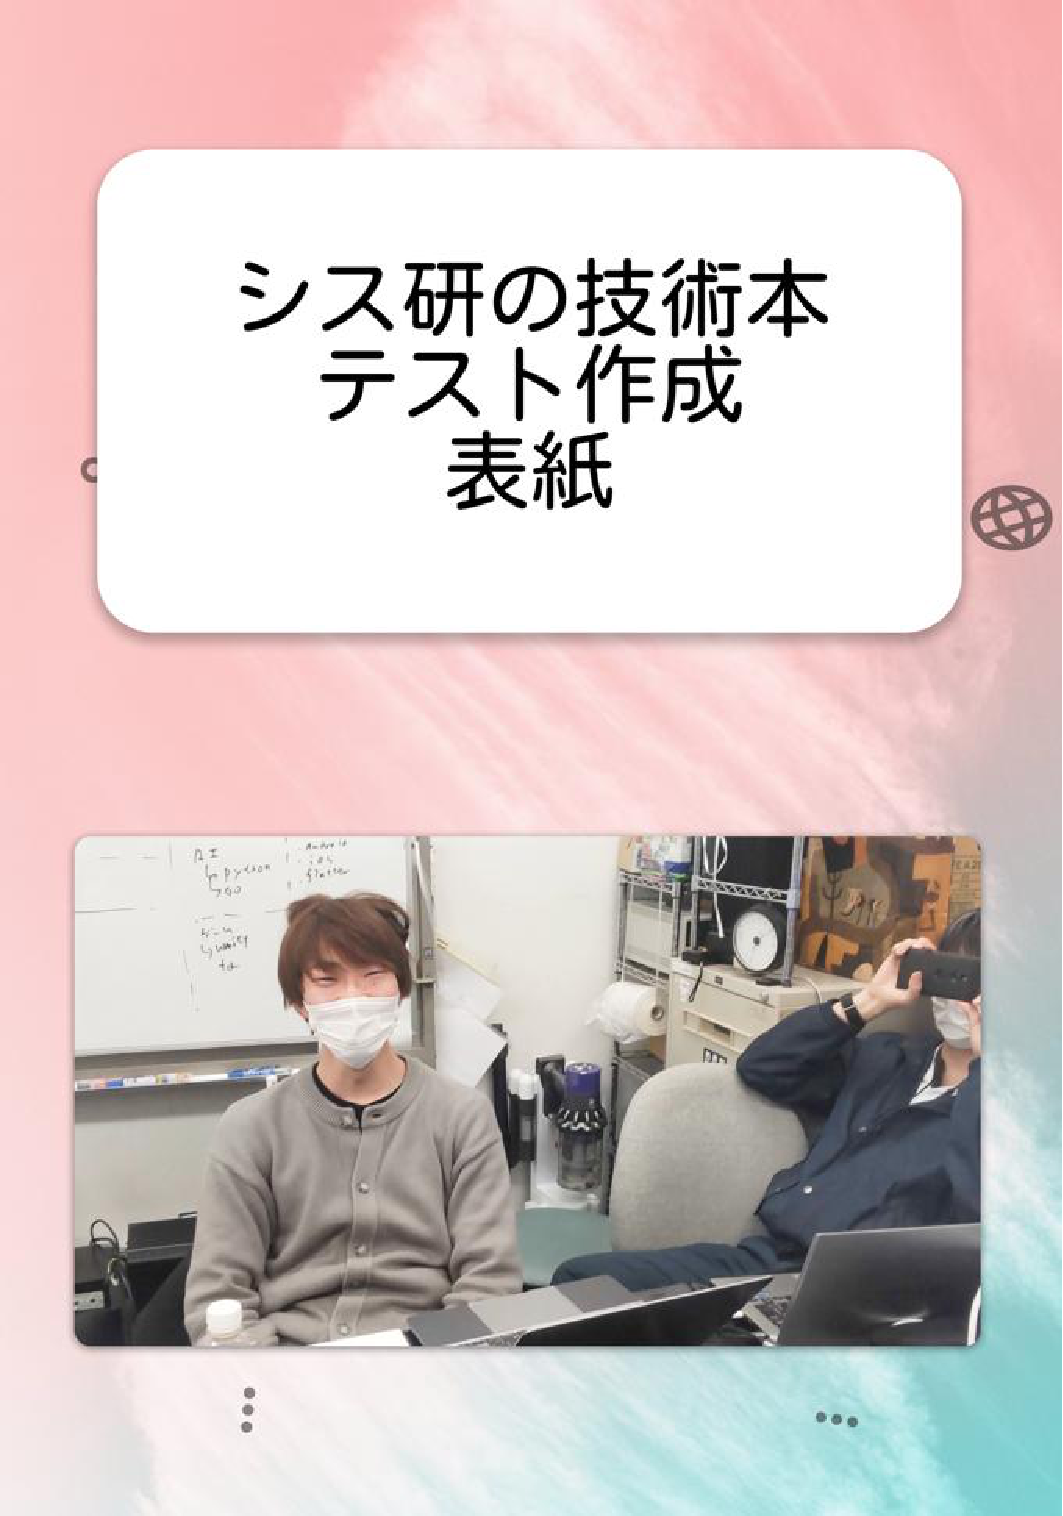
\includegraphics[width=\paperwidth,height=\paperheight]{./image/01-title/titlepage.png}
  \restoregeometry % 元の余白に戻す
\end{titlepage}

%目次を自動的に作る。
\tableofcontents

\chapter{シス研というサークルについて}

\section{シス研というサークルについて}
\subsection{はじめに}
初めまして!シス研会長の林です!
はい、ここでみなさんシス研とはなんぞ?となっていると思うのでまずは自分が水先案内人となりましてこの本とシス研について解説していこうと思います。

\subsection{どんな話をするのか}
シス研ってどんなサークル?どんな活動をしているの?この本はどういったもの?といったものを紹介していきます。それでは、さっそく行ってみましょう!!!

\section{シス研とは}
シス研は正式名称を「システム工学研究会」と言い、愛知工業大学公認の情報系サークルです。歴史は長く、2023年で創立47周年を迎え、かのAppleと同い年となります!! \\
シス研ではハッカソン出場をはじめとしたチーム開発、ゲーム作成、インフラの構築、運用などを行っています。

\subsection{どんな活動をしているの?}
シス研の主な活動はチーム開発とインフラ整備です。サークル全体としての開発物などはなく、それぞれがチームを組んでハッカソンに出場したりしています。 \\
インフラ面では、部室に物理サーバを持っており、そこでシス研のホームページや各種サービスを公開しています。\footnote{シス研ホームページ\url{https://set1.ie.aitech.ac.jp}}\footnote{シス研紹介ページ\url{https://welcome.sysken.net}}23年4月現在、大幅な工事を行なっておりごく一部のサービスのみ稼働しています(すみません)
そのほかにもシス研主催のLT会・ハッカソンの開催、Qiitaアドベントカレンダーへの参加もしています。\footnote{Advent Calendar 2022 \url{https://qiita.com/advent-calendar/2022/stech-ait-advent}}

\begin{figure}[bht]
  \centering
  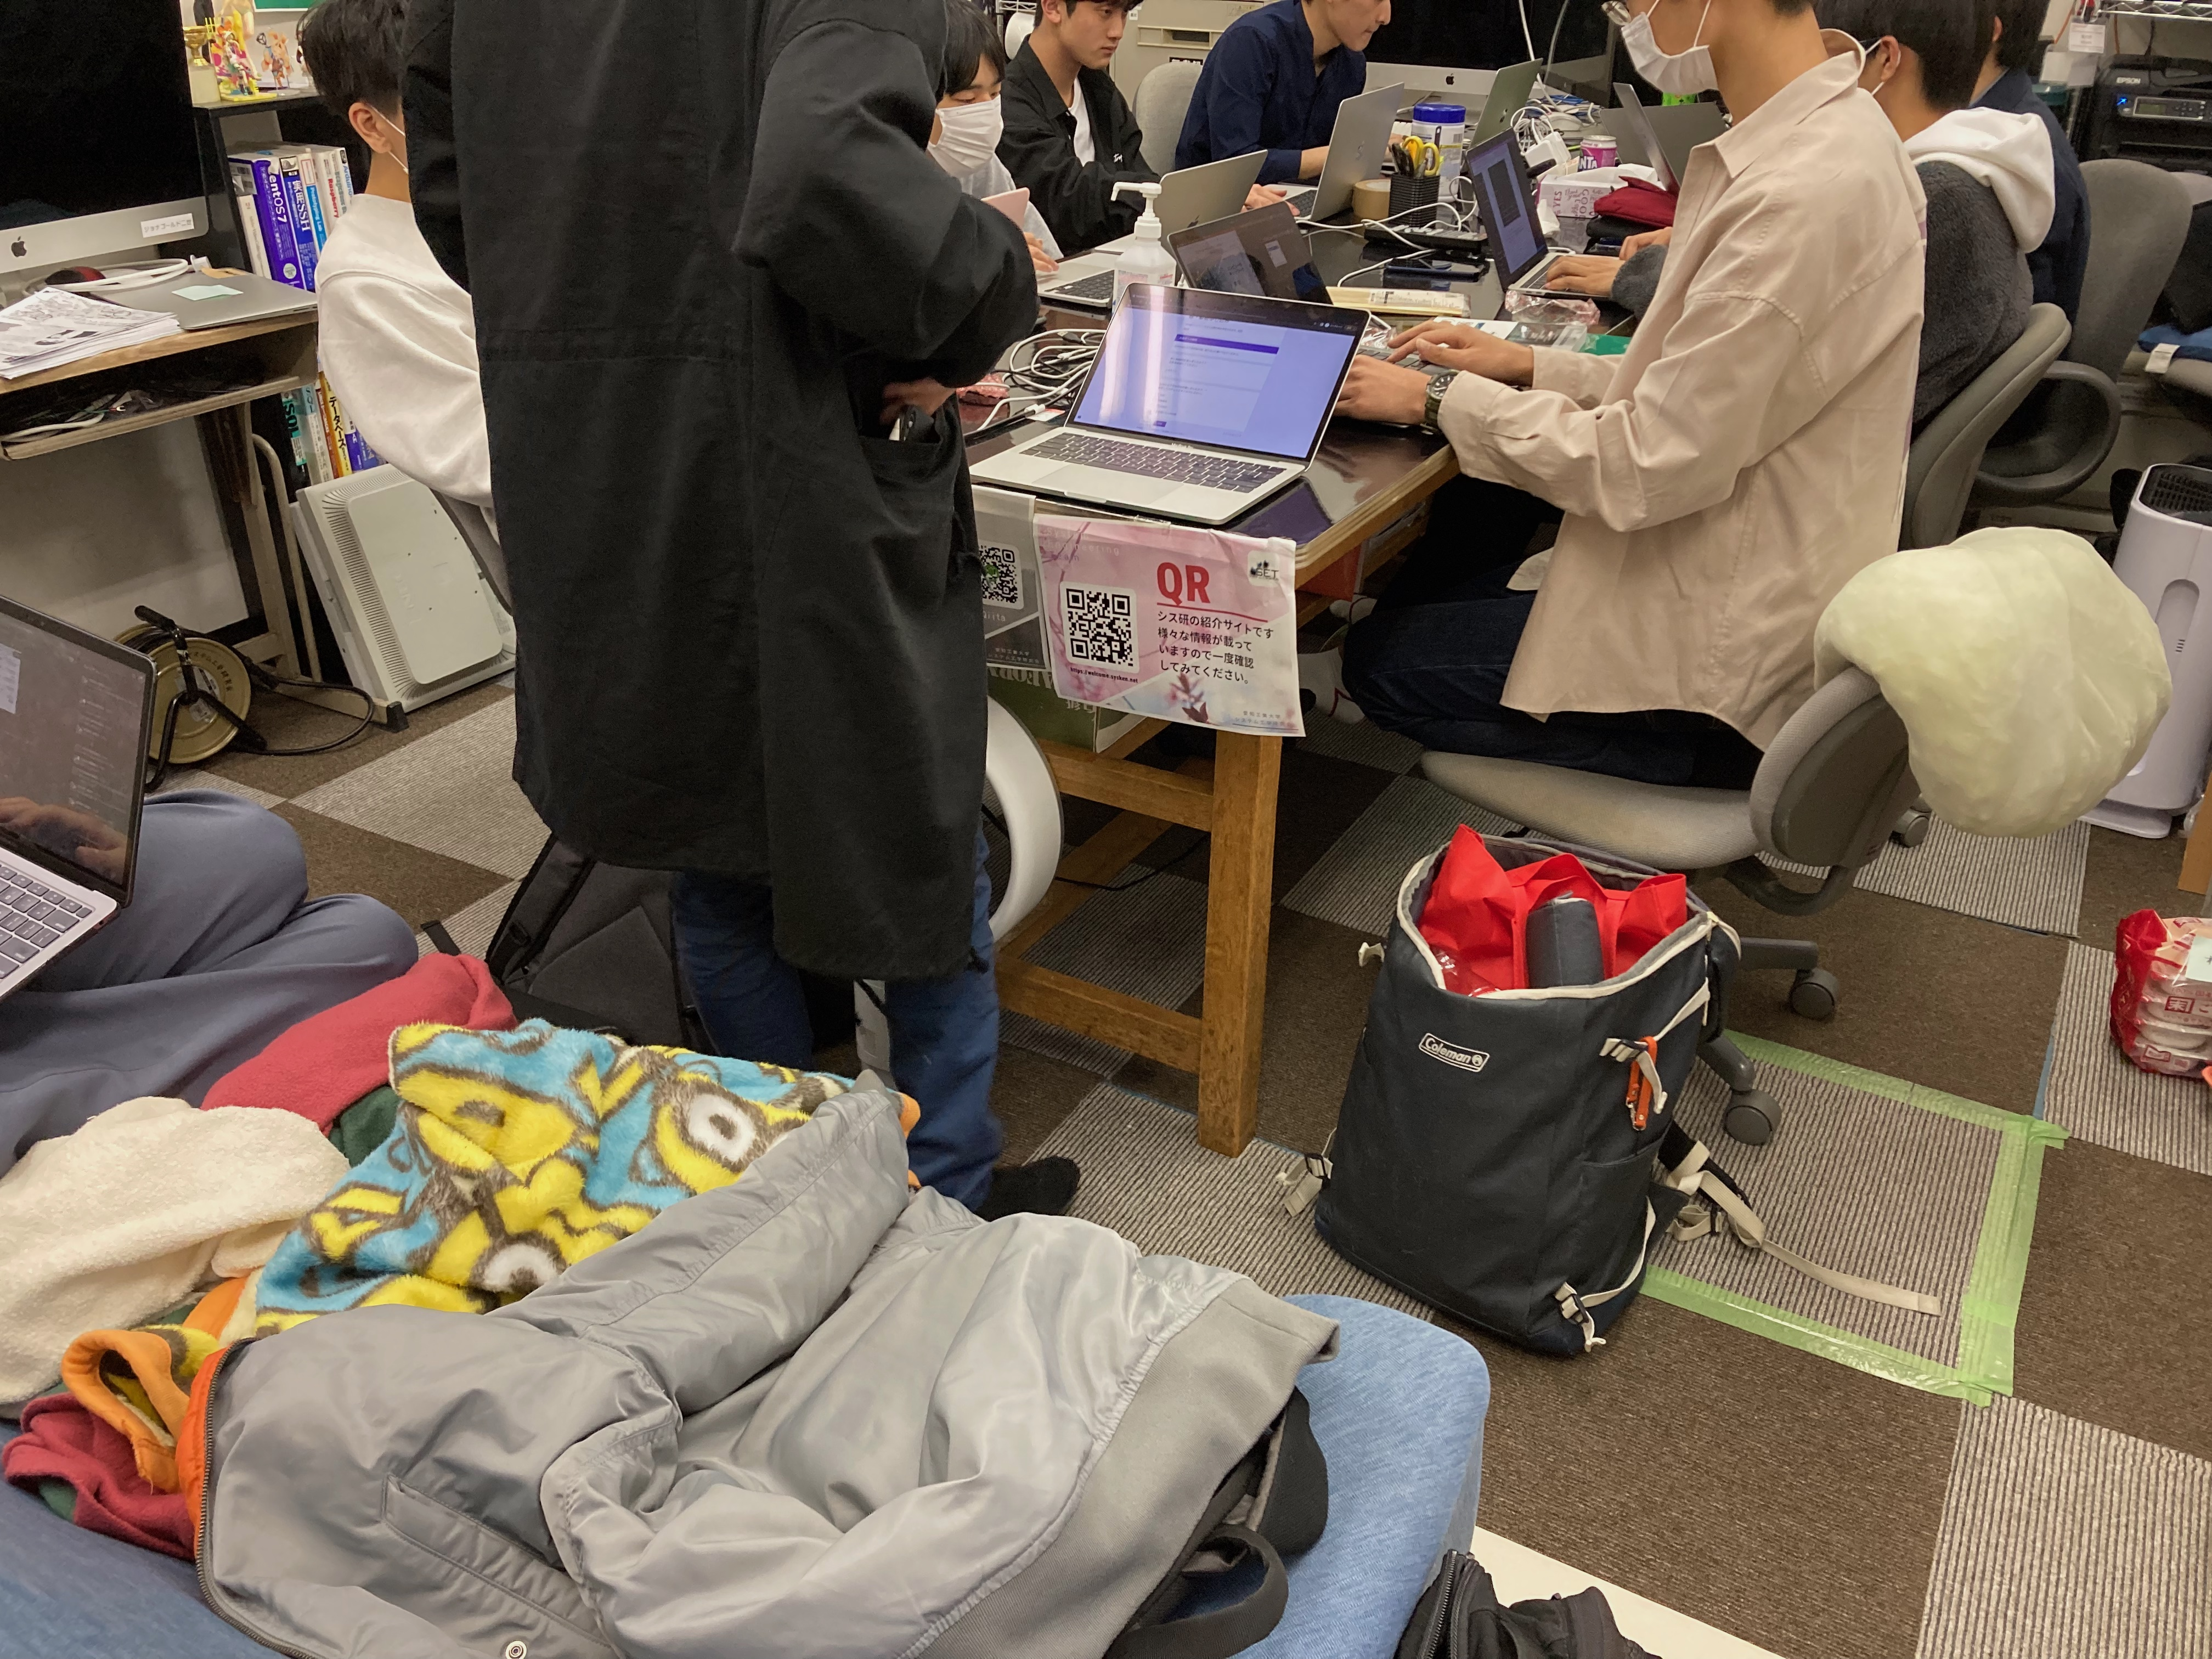
\includegraphics[width=10cm]{./image/02-AboutSysken/room.jpg}
  \caption{部室の様子}
\end{figure}

\subsection{21〜22年度の活動実績}
\begin{itemize}
  \item 2021 愛工大大学祭 工科展 最優秀賞
  \item 2022 技育博 参加
  \item 2022 Geekcamp vol8 優秀賞
  \item 2022 愛工大大学祭 工科展 瑞若賞
  \item 2022 技育展 出展
  \item 2022 愛工大大学祭 模擬店 最優秀賞
  \item 2022 HackU 春・夏 参加
  \item 2022 Geekcampアドバンス 登壇
  \item 長期休暇中のLT会、ハッカソン主催
  \item 各種勉強会の開催
\end{itemize}

\begin{tcolorbox}[title=シス研の設備]
  \begin{itemize}
    \item ブレードサーバ、ネットワーク機器
    \item デスクトップPC
    \item iMac,MacBook
    \item iPhone,iPad
    \item Android端末各種
    \item Raspberry Pi
    \item はんだ等の電子工作セット
    \item その他多数...
  \end{itemize} 
\end{tcolorbox}

\begin{figure}[H]
  \begin{tabular}{cc}
    \begin{minipage}[b]{0.40\columnwidth}
      \centering
      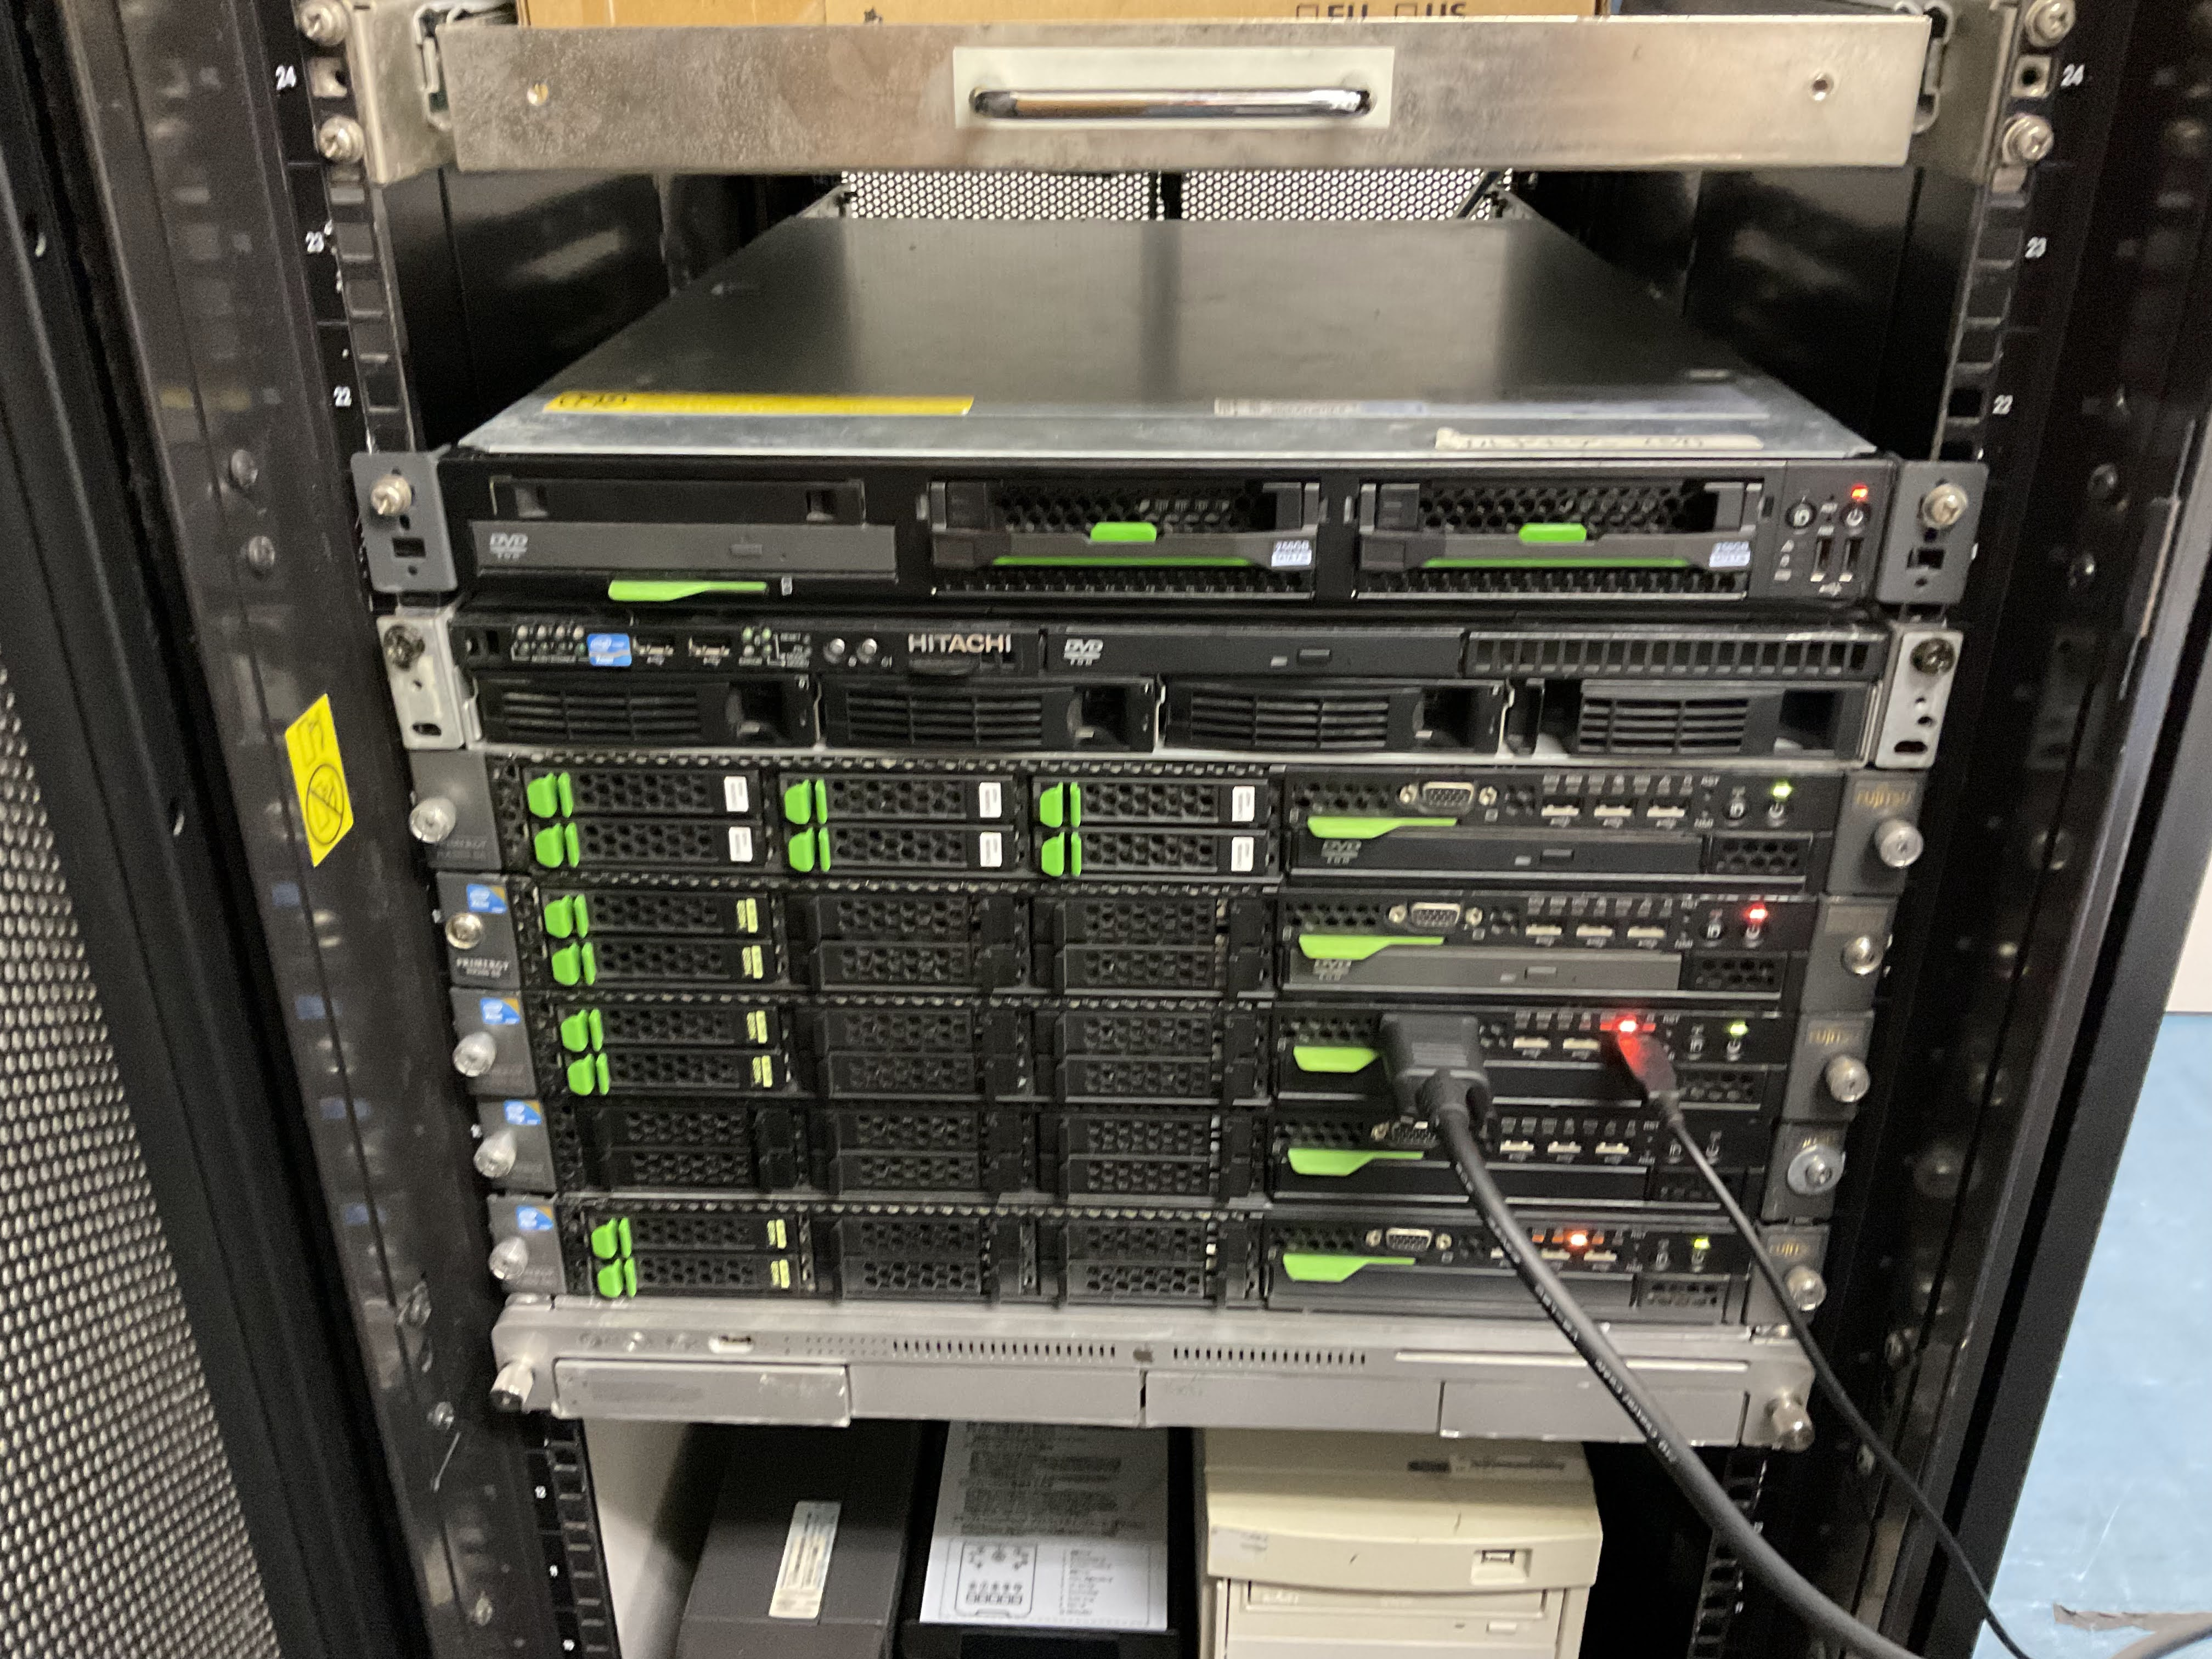
\includegraphics[width=\columnwidth]{./image/02-AboutSysken/server.jpg}
      \caption{ブレードサーバ}
    \end{minipage} &
    \hspace{0.04\columnwidth}
    \begin{minipage}[b]{0.40\columnwidth}
      \centering
      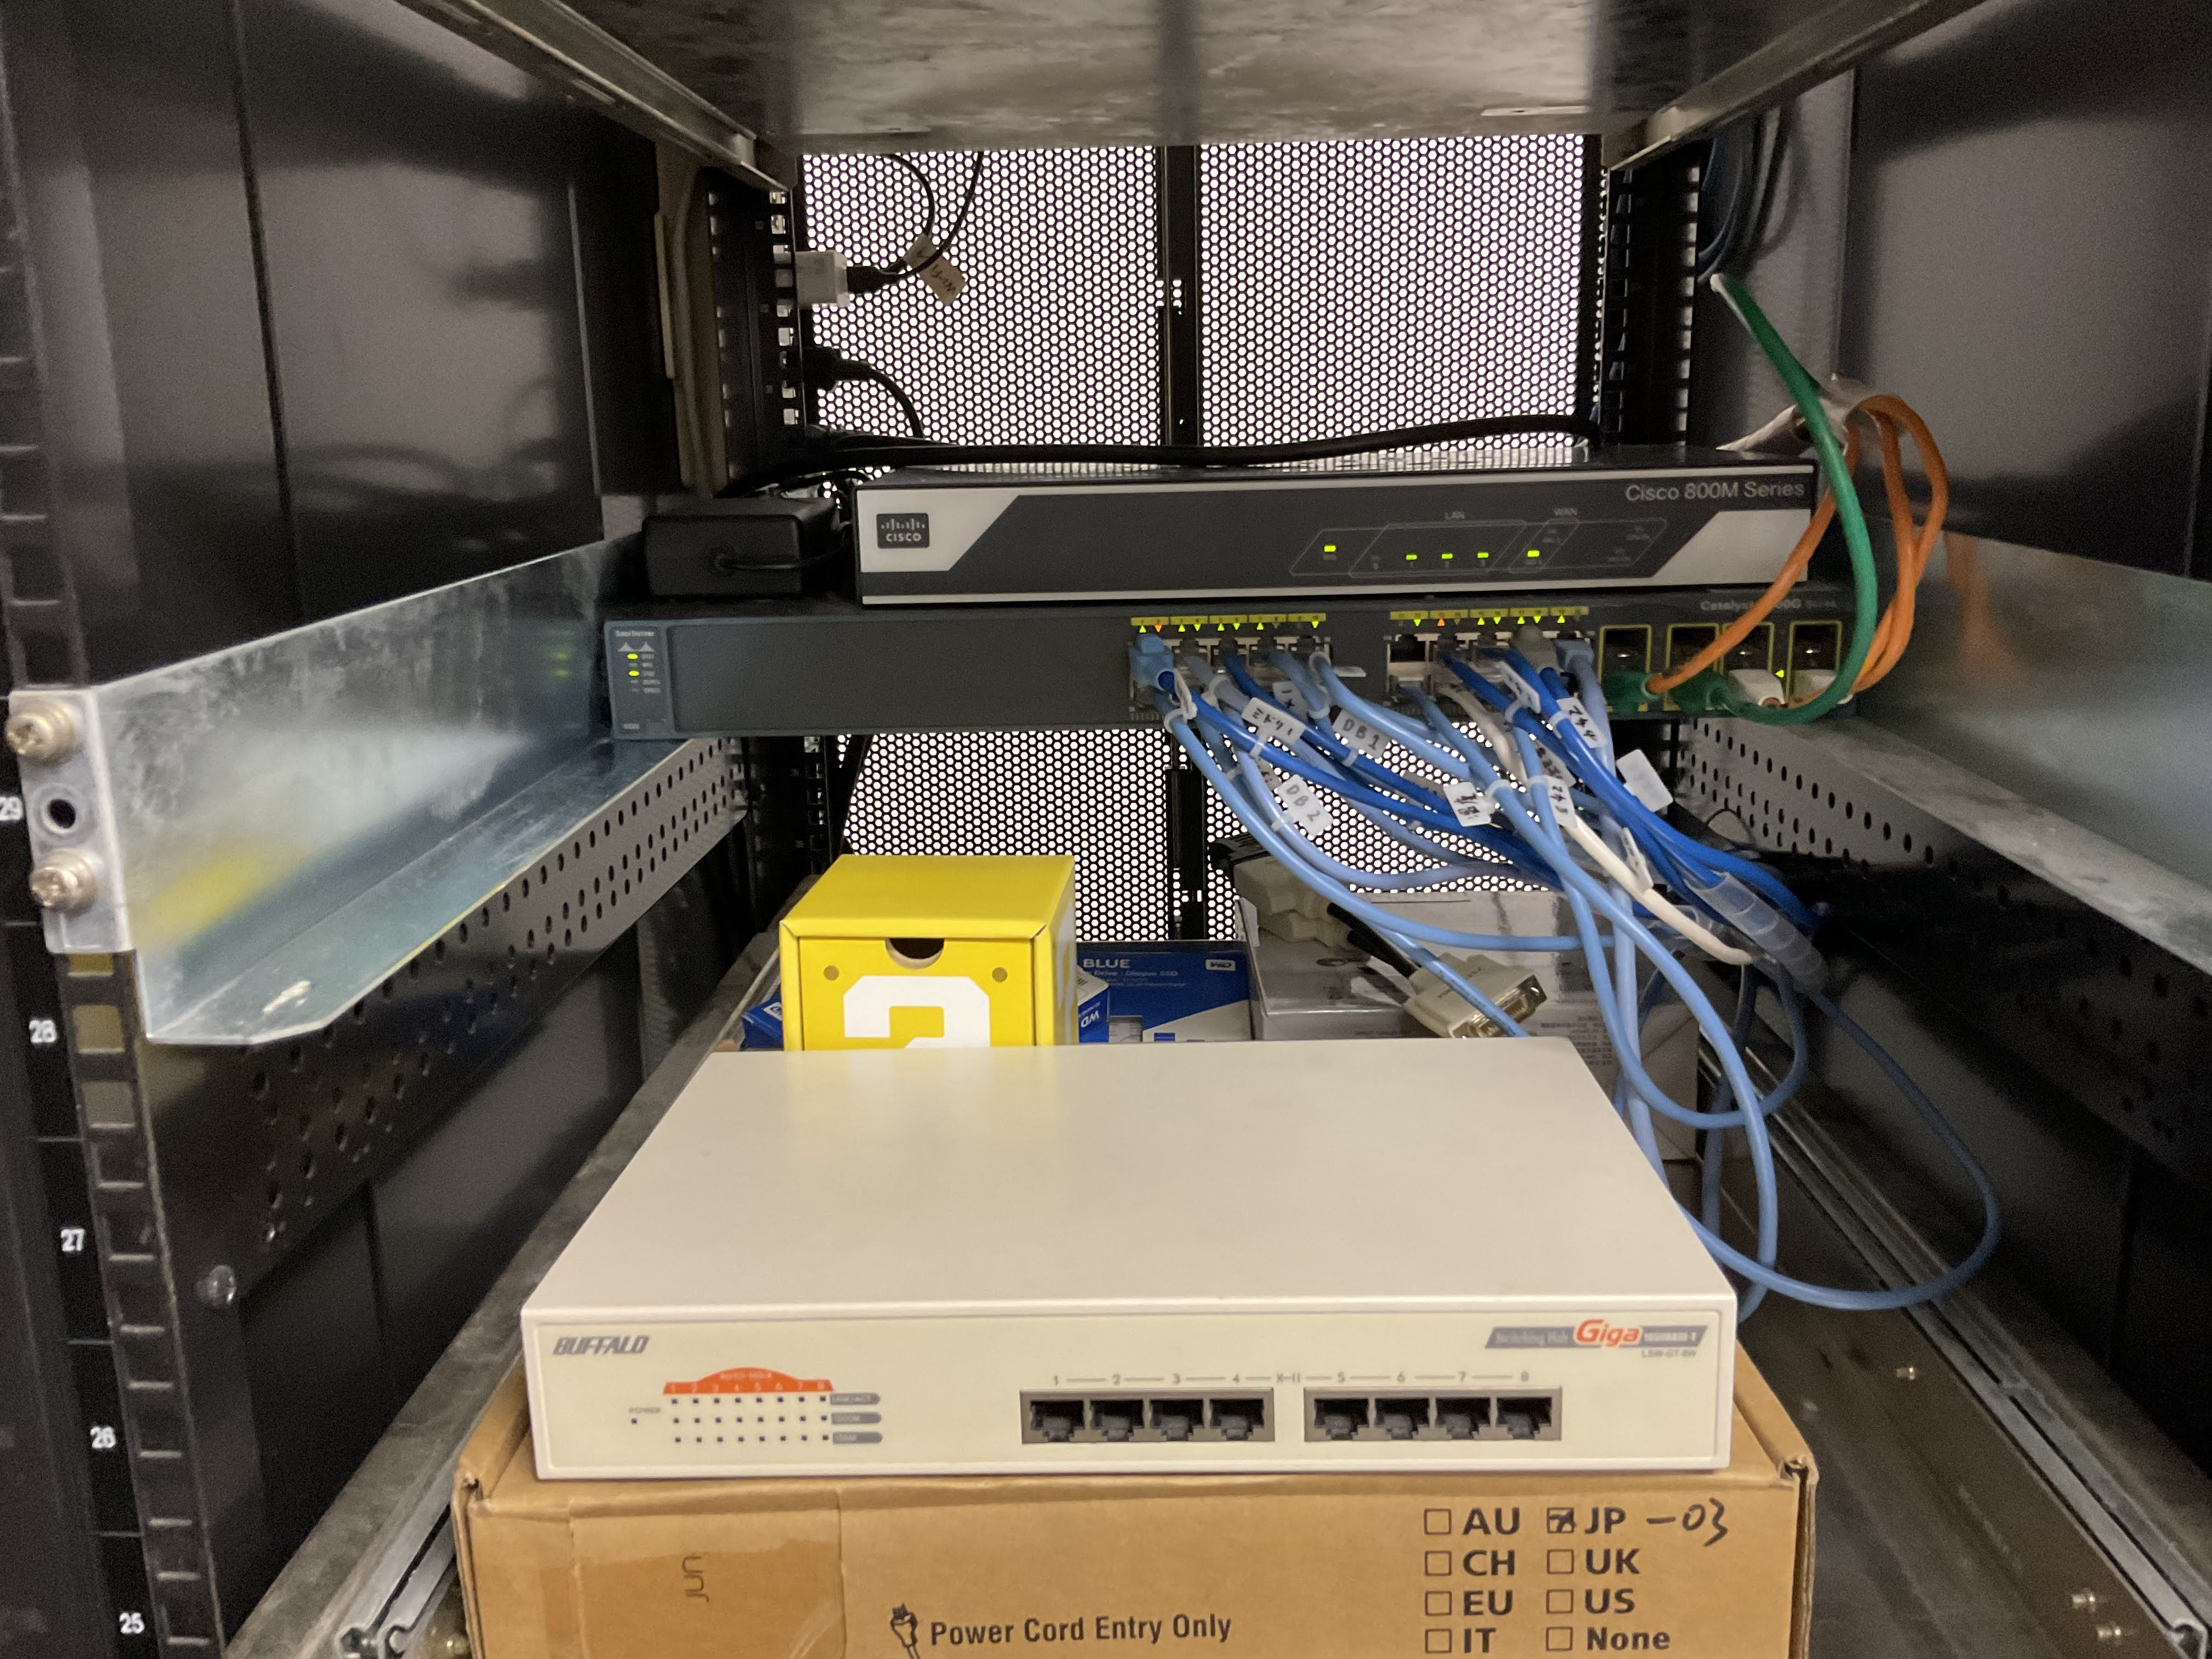
\includegraphics[width=\columnwidth]{./image/02-AboutSysken/network.jpg}
      \caption{ネットワーク機器}
    \end{minipage} \\
    \begin{minipage}[b]{0.40\columnwidth}
      \centering
      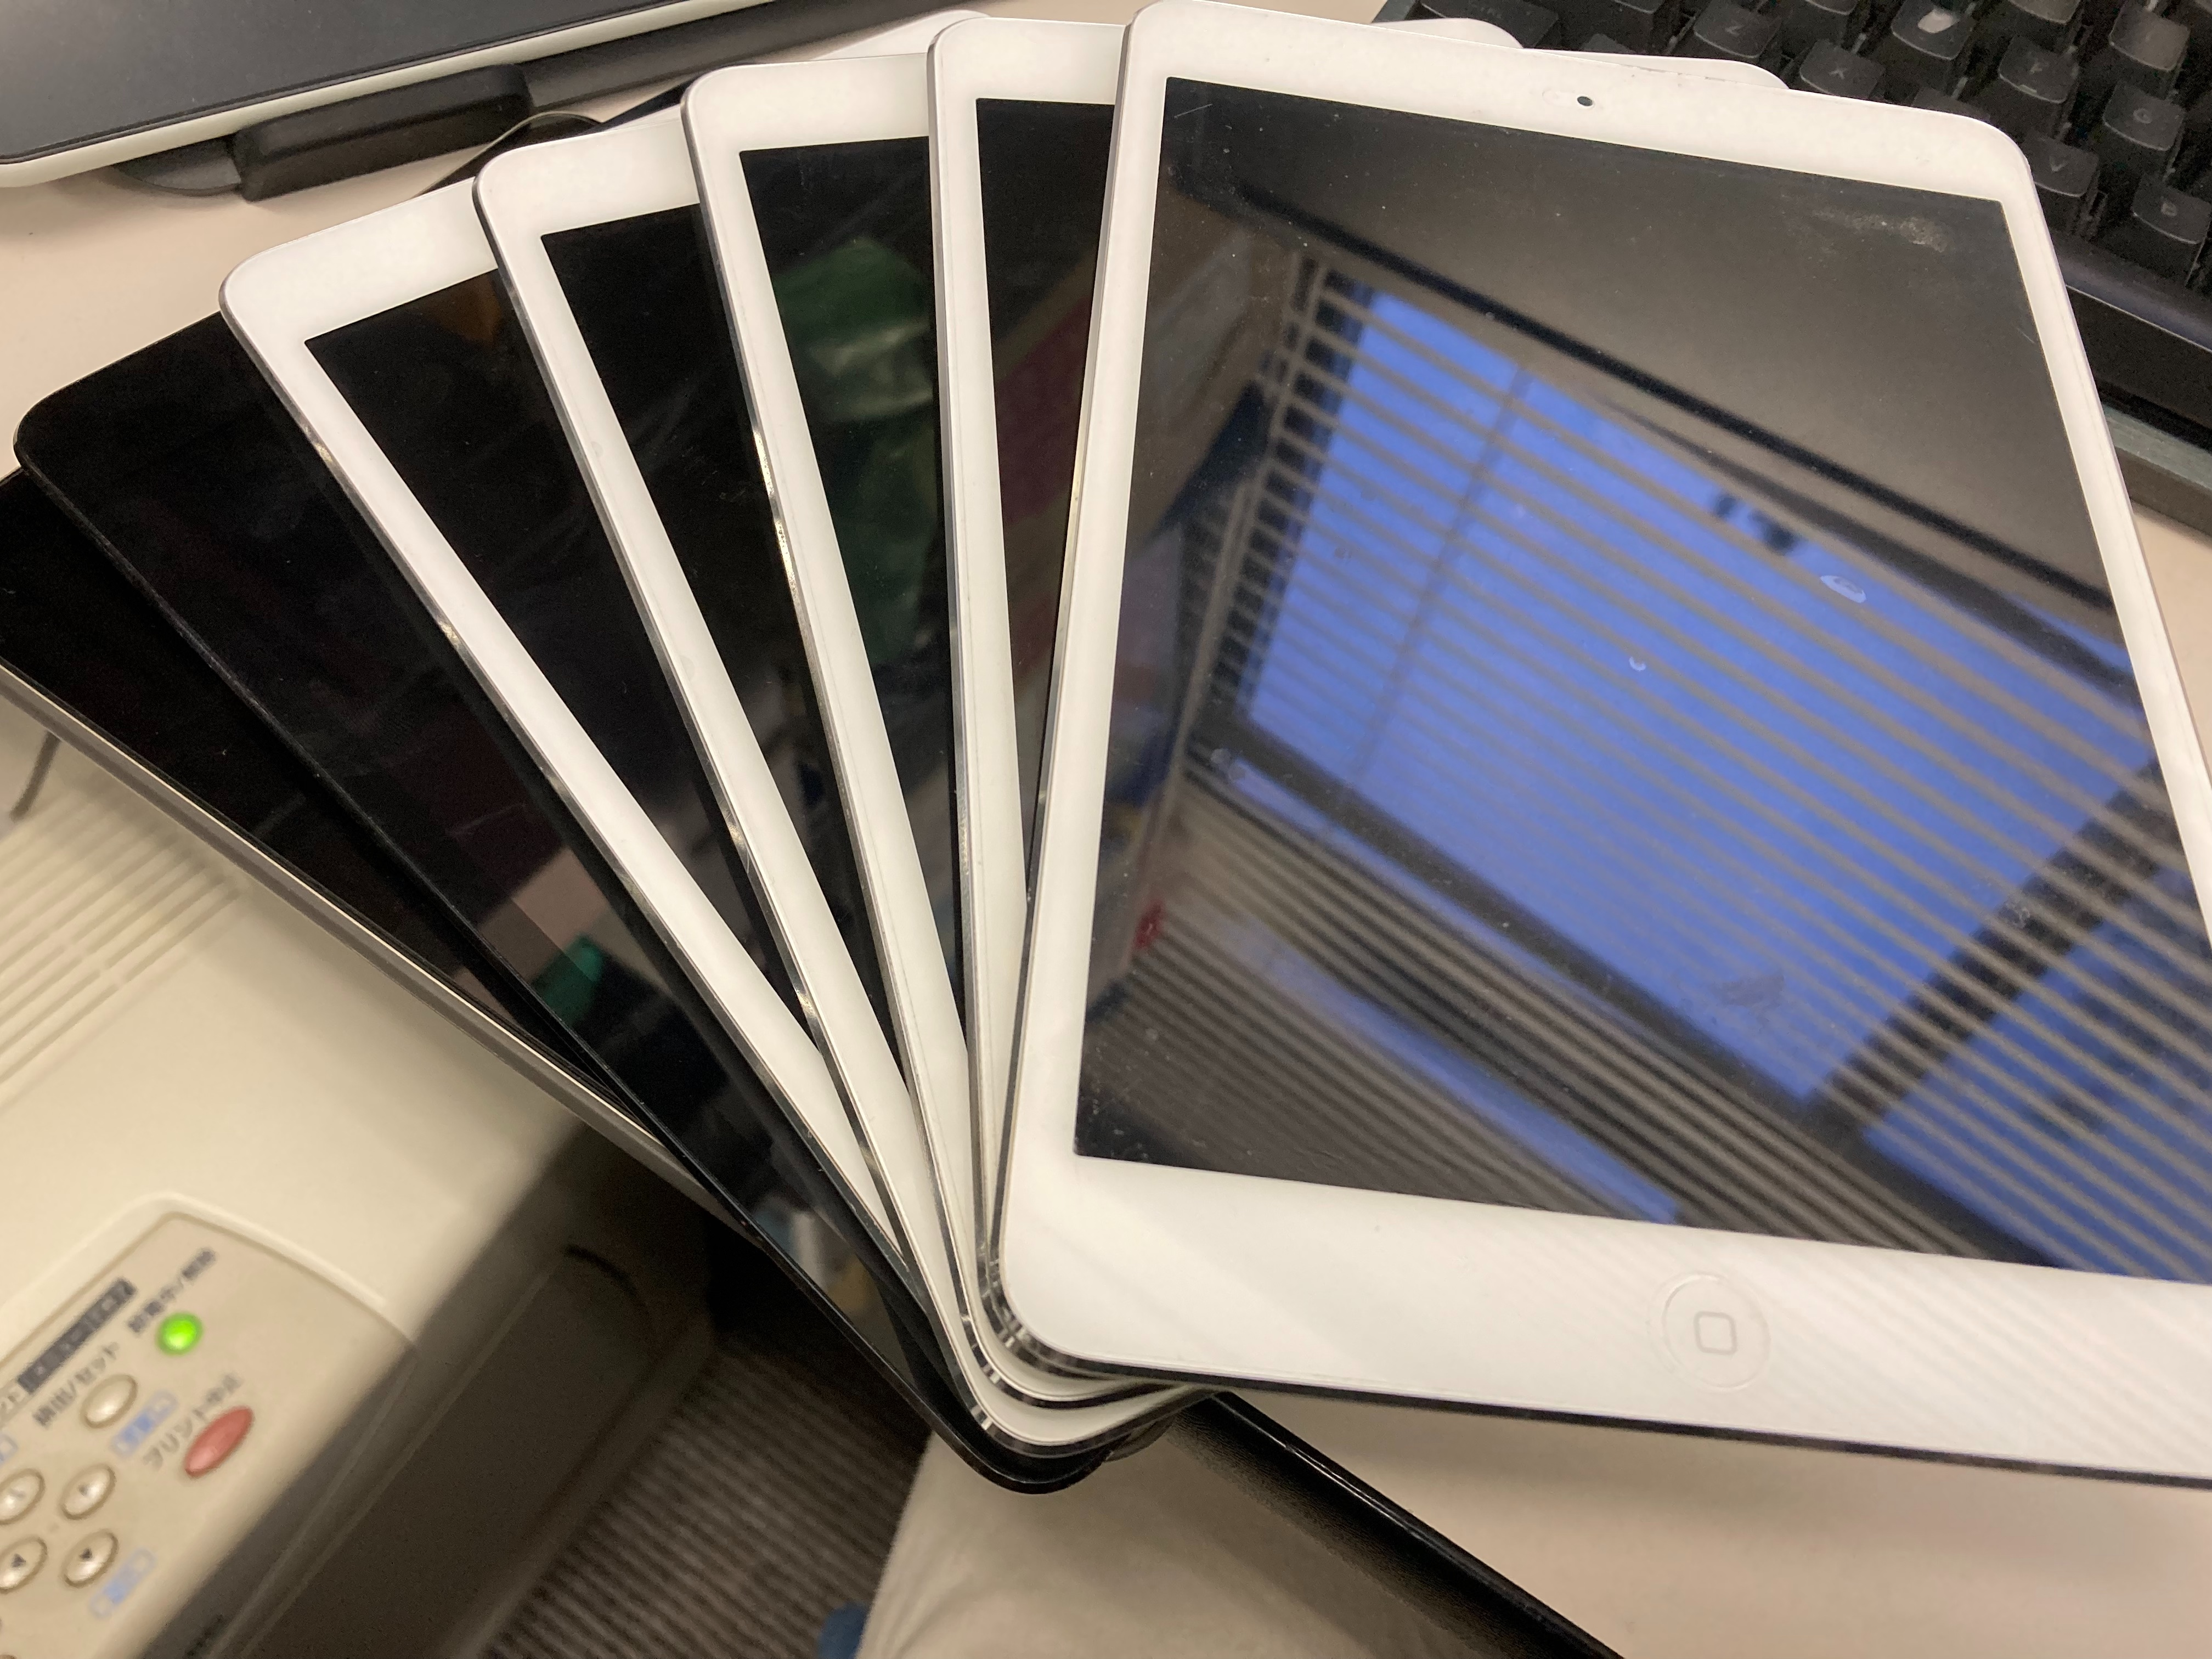
\includegraphics[width=\columnwidth]{./image/02-AboutSysken/iPad.jpg}
      \caption{タブレット端末}
    \end{minipage} &
    \hspace{0.04\columnwidth}
    \begin{minipage}[b]{0.40\columnwidth}
      \centering
      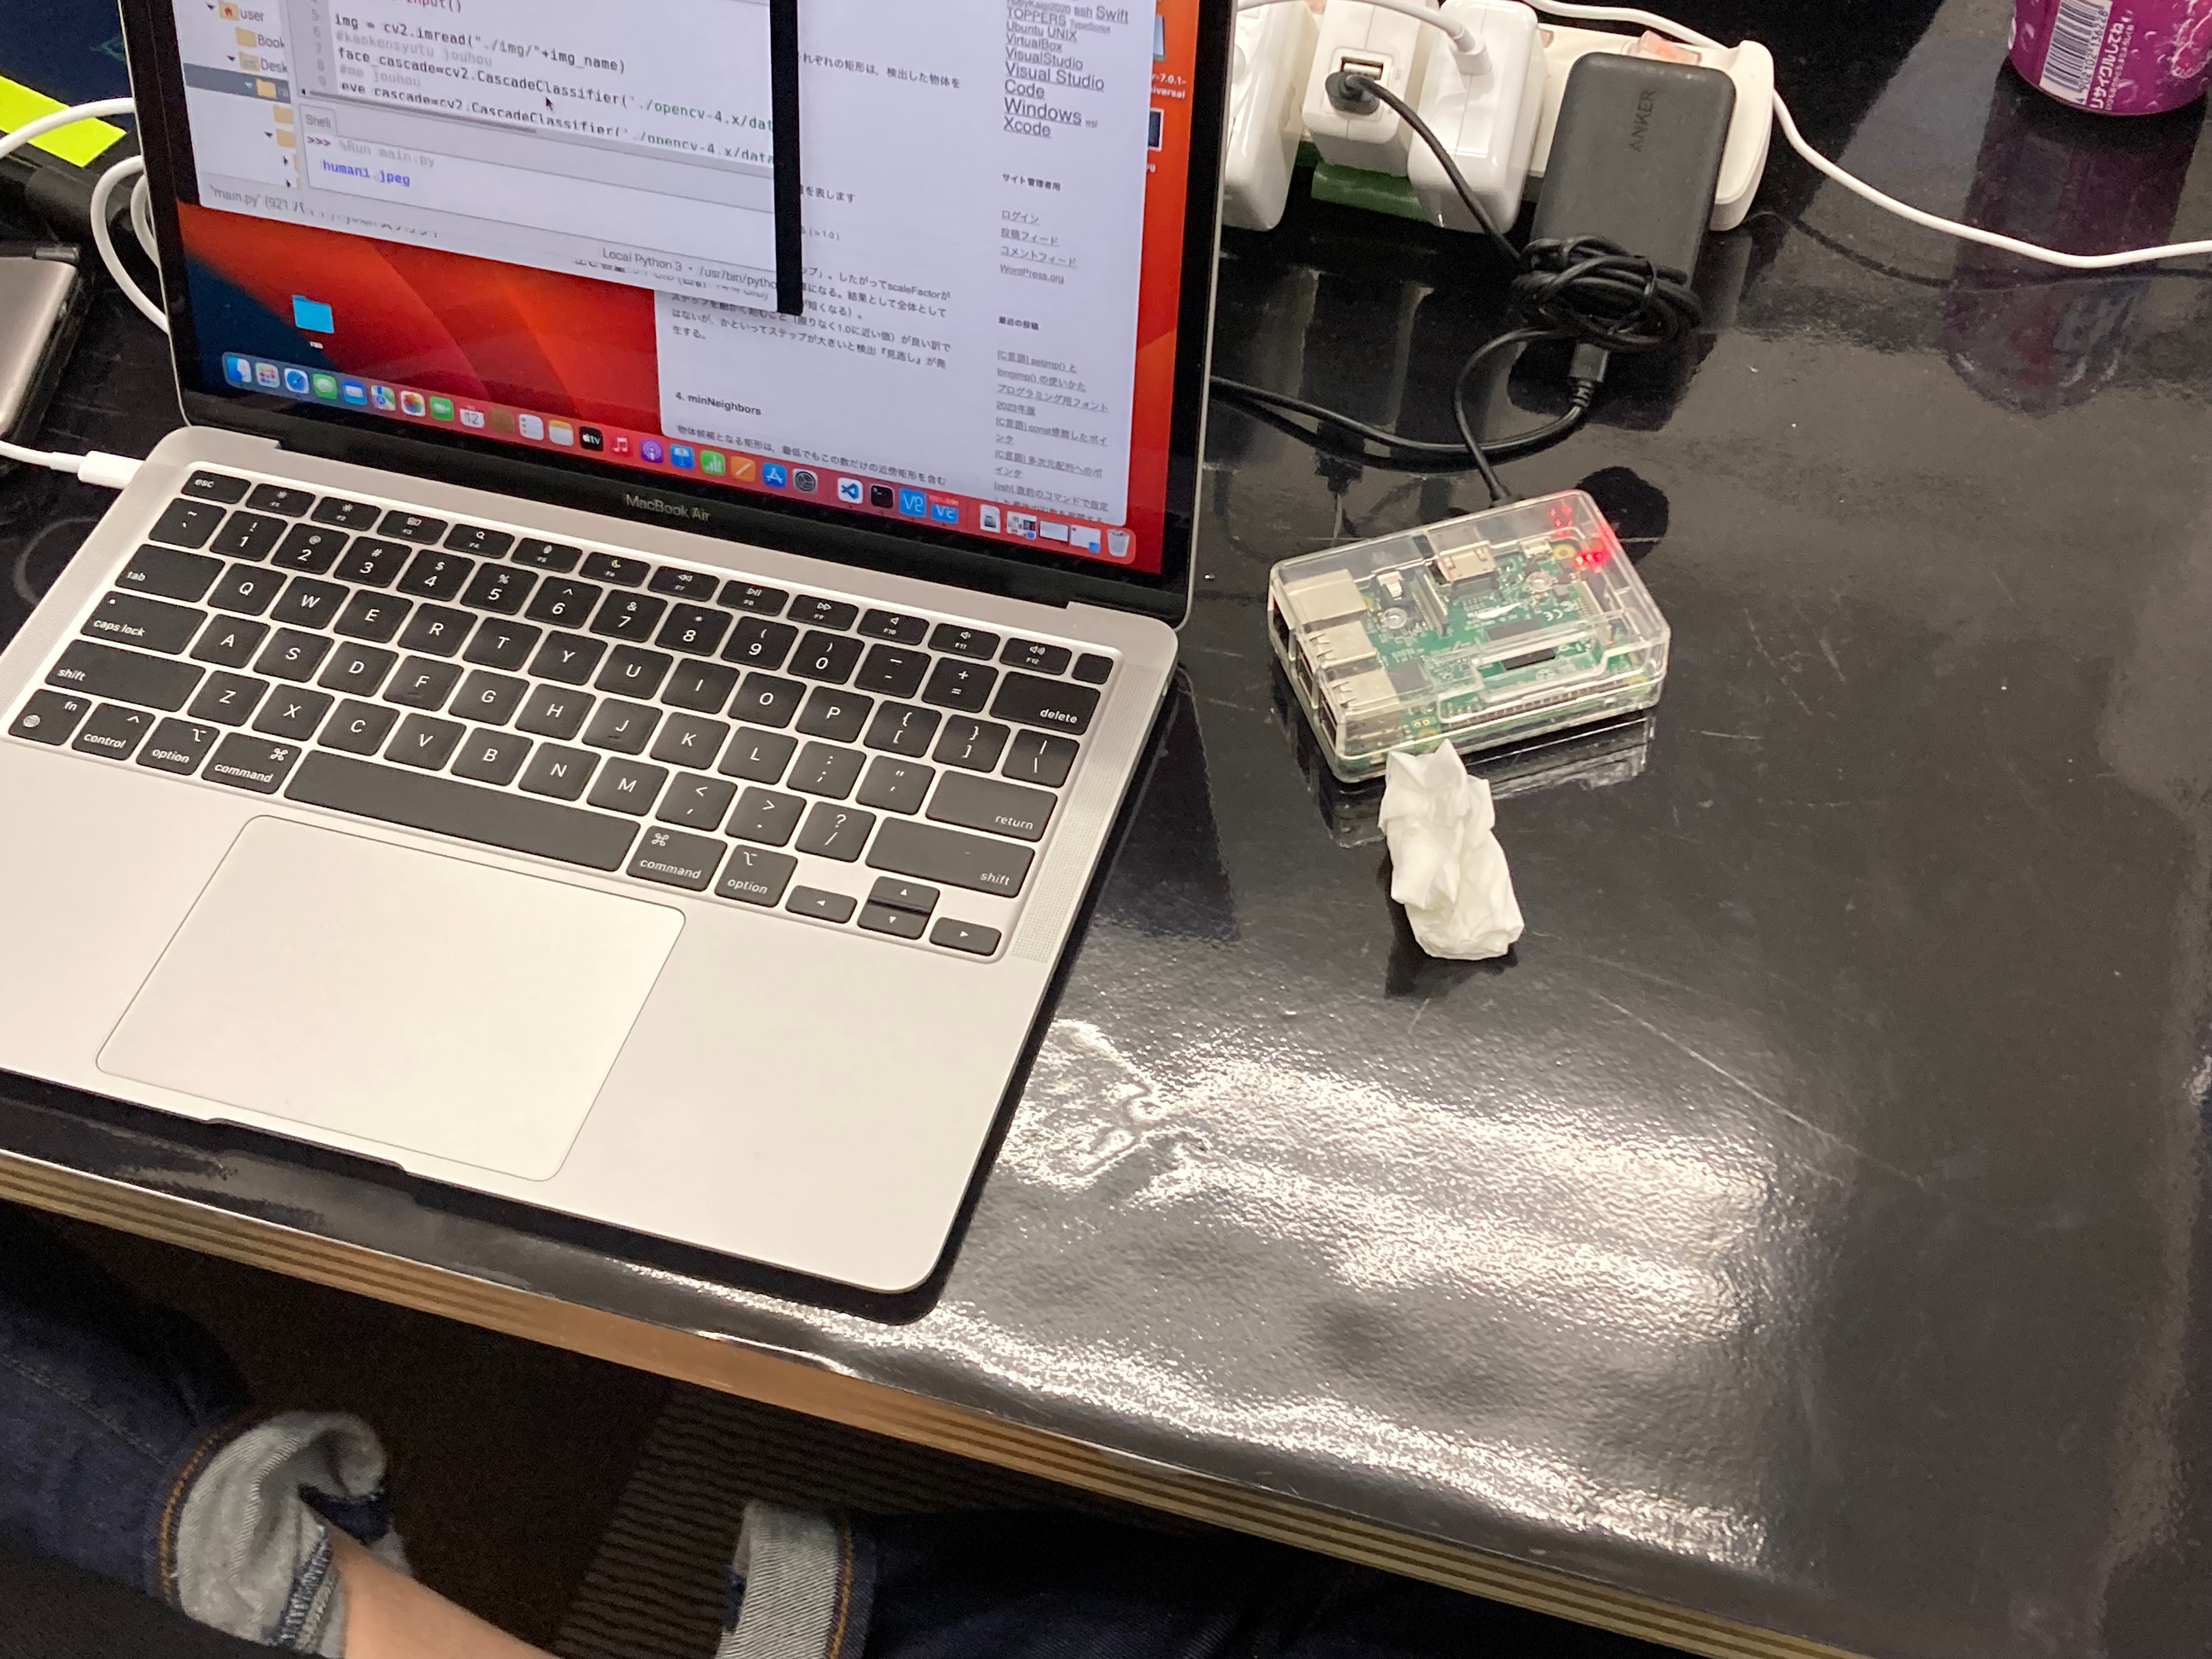
\includegraphics[width=\columnwidth]{./image/02-AboutSysken/RaspberryPi.jpg}
      \caption{Raspberry Pi}
    \end{minipage}
  \end{tabular}
\end{figure}

\section{この本について}
この本はシス研のメンバーが経験したこと、取り組んだことのアウトプットを目的としたものです。この本を通じて皆さんにはシス研のメンバーは具体的にどのような活動をしているのか知ってもらいたいと思います。 \\
また、シス研として本を出すのは今回が初めてなのでどうか温かい目で見ていただけると幸いです。

\section{まとめ}
ここまでお話をして来ましたが簡単にでもシス研について知ってもらうことはできたでしょうか?うまく伝えることができていたらとても嬉しいです。 \\
次のページからはメンバーの記事本編になります!シス研初めての本をよろしくお願いします!!
\chapter{DiscordBotを作ってみよう!}

\section{DiscordBotを作ってみよう}
\subsection{はじめに}
はじめまして、sudaです。私はDiscordで人とチャットをしている時に同じ会話が頻繁に続き、これBotで返事をするようにしたら返事をする手間が省けるし面白いのでは?と思いBotを作ることにしました。
発想がひどいって!?まあでも自分の発想したものを形にすることが面白いことだと思うので今回はそこには目を瞑りましょう…
もちろん自分が送ったメッセージに対してBotに返答させることもできるので、自分だけのオリジナルDiscordBotを作ってみましょう!

\subsection{何を作るのか}
Discordのサーバで特定のメッセージが来たら、特定のメッセージを返すDiscordのBotを作ります。
サンプルプログラムを参照したい方は以下のURLからご覧下さい。
\footnote{今回作るDiscordBotのサンプルプログラム\url{https://github.com/sudamichiyo/Discord_Bot_sampleprogram}}
例えば自分が「仕事終わった」と言うとBotが「お疲れ様」と返してくれます。
\section{実行環境・使用技術}
\begin{itemize}
  \item Python 3.10.8
\end{itemize}


\section{ローカル環境でBotが動作するようにする}
まずはローカル環境でBotが動作するようにしてみます。

\subsection{Botの作成・管理をする}
初めに、機能などはまだついていないBotをDiscordのポータルサイトから作成します。
DiscordのBotの作り方(メモ)という記事の「1.Discord上のBotの作成」を見ながらBotを作成してみて下さい。
\footnote{DiscordのBotの作り方(メモ)\url{https://note.com/exteoi/n/nf1c37cb26c41 (参照2023.3.29)}}

\subsection{ファイルの作成}
Botを実行するPythonファイルを作ります。
\begin{shaded}
  \begin{verbatim}
$ mkdir message_discord_bot
$ cd message_discord_bot
$ touch main.py
\end{verbatim}
\end{shaded}

\subsection{discord.pyの準備}
ここからはdiscord.pyのドキュメントを見ながら環境構築をしていきます。
\footnote{discord.pyドキュメント\url{https://discordpy.readthedocs.io/ja/latest/intro.html\#basic-concepts (参照2023.3.29)}}
PythonでDiscordのAPIを操作するために必要なライブラリをインストールします。先ほど作成したディレクトリにアクセスして、以下のコマンドで discord.py をインストールします。
\begin{shaded}
  \begin{verbatim}
$ python -m pip install -U discord.py
\end{verbatim}
\end{shaded}
次に、先ほど作成したmain.pyを以下のソースコードに書き換えます。
\begin{tcolorbox}[breakable]
  \begin{verbatim}
1 import discord
2 
3 class MyClient(discord.Client):
4     async def on_ready(self):
5         print(f'Logged on as {self.user}!')
6 
7     async def on_message(self, message):
8         print(f'Message from {message.author}
9                                         : {message.content}')
10
11 intents = discord.Intents.default()
12 intents.message_content = True
13
14 client = MyClient(intents=intents)
15 client.run('my token goes here')
\end{verbatim}
\end{tcolorbox}
ここで、以下のボットに関する2つの設定をDiscordのポータルサイトから設定してください。
\begin{itemize}
  \item ポータルサイトの「Bot」からトークンを取得する
  \item ポータルサイトの「Bot」の「MESSAGE CONTENT INTENT」を有効にする
\end{itemize}
'my token goes here'は取得したBotのアクセストークンを書きます。
以上の設定が終わったところで python3 main.py を実行すると、Botのサーバが立ち上がります。Botサーバ起動後にBotのいるサーバでメッセージを投げると、コマンドライン上に「書いた人」と「メッセージ」がそのまま出力されます。

\subsection{環境変数の設定}
ソースコードに直接トークンを書いてしまうと、Githubでソースコードをホスティングするときにトークンキーが他の人にバレてしまいます。
これを防ぐために.envファイルを作成して、その中にDiscordのアクセストークンを書きます(下記参照)。
\begin{tcolorbox}[breakable]
  \begin{verbatim}
1 DISCORD_TOKEN='My token goes here'
\end{verbatim}
\end{tcolorbox}
Pythonの中で.envファイルに書かれている変数を取得するために dotenv というライブラリを使用します。以下のようにインストールします。
\begin{shaded}
  \begin{verbatim}
$ pip install python-dotenv
\end{verbatim}
\end{shaded}
インストール後にmain.pyに下記のコードを付け加えて下さい。\\
main.pyのimport discordとclass MyClientの間に以下のコードを追加します。
\begin{tcolorbox}[breakable]
  \begin{verbatim}
1 import os
2 from dotenv import load_dotenv
3 load_dotenv()
\end{verbatim}
\end{tcolorbox}
そして、最後の行を以下のように書き換えて下さい。
\begin{tcolorbox}[breakable]
  \begin{verbatim}
1 client.run(os.environ['DISCORD_TOKEN'])
\end{verbatim}
\end{tcolorbox}
書き換えたあとに python3 main.py を実行すると,先ほどと同じようにメッセージの受け取りをしてくれるサーバーサイドアプリケーションが立ち上がります。

\subsection{Botが特定のワードに反応して、特定のメッセージを返答する機能をつける}
プログラムを起動して正常にサーバーサイドアプリケーションがメッセージを受け取れるようになったら、Botが特定のワードに反応して、特定のメッセージを返答する機能をつけていきます。
Botに機能をつけるには上記のソースコードの8行目と10行目の間に以下のコードを付け足していきます。\\
\begin{tcolorbox}[breakable]
  \begin{verbatim}
1 # メッセージを書いた人がBotなら処理終了
2 if message.author.bot:
3     return
4 channel = message.channel 
5 if message.content == '仕事終わった':
6     await channel.send('お疲れ様')
\end{verbatim}
\end{tcolorbox}
付け足したコードの解説をしていきます。\\
2,3行目でメッセージを書いた人がBotなら処理を終了させています。\\
4行目でメッセージが投稿されたチャンネル取得しています。\\
5行目のmessage.contentはメッセージの内容で、今回の場合「仕事終わった」というメッセージをチャンネルに投稿すると、メッセージが投稿されたチャンネルにBotが「お疲れ様」と返答します。
\section{まとめ}
今回はDiscordのBotの作り方を説明しました。上記の「仕事終わった」や「お疲れ様」に当たる部分を変えたりして自分好みに改良してみて下さい。
\chapter{リポジトリ作成後に設定しておきたいこと}
\section{はじめに}
こんにちは。hihumikanです。

本チャプターでは「リポジトリ作成後に設定しておきたいこと」をご紹介します。
私自身が次回プロジェクト開始する際に、こういった設定や技術を使うだろうというものをまとめました。

ただし、これら全ての内容をプロジェクトに適用出来るものではないため、ご利用の環境や用途に合わせて利用していただければと思います。

\subsection{対象読者}

対象読者は、Git/GitHubを利用した開発を行う初学者の方を想定しています。

\section{ファイルの設定}

リポジトリ作成後に設定しておきたい「ファイルの設定」についてご紹介します。

\subsection{.gitignore}

.gitignoreは、Gitによる管理から除外したいファイルやディレクトリを指定するための設定ファイルです。

例えば、MacOSの場合、ディレクトリ毎に.DS\_Storeというファイルが自動的に生成されます。
このファイルは、ディレクトリのmeta情報を記録しますが、通常の開発において共有する必要がないため、Gitの管理対象外としておくことが望ましいです。

また、.envなどの環境変数を利用してプログラムを動かす場合、.envファイルには、パスワードや秘密鍵などの情報が含まれていることが多いため、これもGitの管理対象外としておくことが望ましいです。

リスト1.1のようなテキストファイルをGitの管理下に置くだけで、Gitから管理対象外として扱うことができます。

\begin{tcolorbox}[title=リスト1.1 .gitignore]
  \begin{verbatim}
1 .DS_Store
2 .env
\end{verbatim}
\end{tcolorbox}

リポジトリを共有する場合、.gitignoreファイルを共有することで、開発メンバー全員が同じ設定を利用できるため、必要なファイルだけがGitの管理下に置かれるようになります。

\subsection{.gitattributes}

.gitattributesは、特定のファイルに対してGitの挙動を変更するための設定ファイルです。
主に、改行コードやファイルの文字コードを指定するために利用されます。

改行コードを指定する理由としては、WindowsとMacOSでは改行コードが異なることが挙げられます。
Gitで管理されているファイルの改行コードが一致しないと、差分が発生してしまい、想定した挙動と異なる動作をすることがあります。
それを防ぐために、.gitattributesに改行コードを明示しておくことで、安全に開発を進めることができます。

リスト1.2のように、ファイルの拡張子に対して、改行コードを指定することができます。

\begin{tcolorbox}[title=リスト1.2 .gitattributes]
  \begin{verbatim}
1 * text=auto
2 *.sh text eol=lf
\end{verbatim}
\end{tcolorbox}

これも.gitignoreと同様に.gitattributes共有することで、開発メンバー全員が同じ設定を利用することができます。


\subsection{Makefile}

Makefileは、コマンドをまとめて実行するための設定ファイルです。

利点として、開発メンバー全員が同じコマンドを実行することができることが挙げられます。
環境構築やテストの実行など、手順が複雑な作業を一人一人が実行した場合、手順の違いによるエラーが発生する可能性があります。
それらを防ぐために、Makefileにまとめておくことで、開発メンバー全員が同じコマンドを実行することができ、人的ミスを防ぐことができます。

Makefileの例としては、リスト1.3のようなものです。

\begin{tcolorbox}[title=リスト1.3 Makefile]
  \begin{verbatim}
1 up: ## APIとデータベースを起動
2   docker compose -f docker-compose-db.yml -p db up -d
3   docker compose -f docker-compose-api.yml -p api up -d
4 
5 build: ## サービスの構築
6   docker compose -f docker-compose-db.yml -p db build
7   docker compose -f docker-compose-api.yml -p api build
8 
9 stop: ## サービスを停止
10   docker compose -f docker-compose-db.yml -p db stop
11   docker compose -f docker-compose-api.yml -p api stop
12 
13 kill: ## サービスを強制停止
14   docker compose -f docker-compose-db.yml -p db kill
15   docker compose -f docker-compose-api.yml -p api kill
16 
17 down: ## サービスの停止とコンテナの削除
18   docker compose -f docker-compose-db.yml -p db down
19   docker compose -f docker-compose-api.yml -p api down
20 
21 restart: ## サービスの再起動
22   docker compose -f docker-compose-db.yml -p db restart
23   docker compose -f docker-compose-api.yml -p api restart
 \end{verbatim}
\end{tcolorbox}

これらを実行する場合、シェルに
\begin{shaded}
  \begin{verbatim}
$ make up
\end{verbatim}
\end{shaded}
と入力することで、2,3行目のコマンドが実行されます。
リスト1.3の例は簡単なものですが、他にもMakefile内に変数を定義することが出来るため、変更が必要な箇所を変数に置き換えることで、コマンドの変更を容易に行うことができます。

\section{インフラ回り}

\subsection{GitHub Actions}
Github Actionsは、GitHub上で動作するCI/CDツールです。
簡単に言えば、仮想マシン上でコマンドを実行することができるものです。

用途としては、コードの静的解析やテストの実行、デプロイなどが挙げられます。
その他にも、Pull Requestに対して、テスト内容をコメントすることができる等のGitHub上での機能を利用することができます。

利用方法としては、リスト1.4のように、.github/workflowsディレクトリを作成し、その中に設定ファイルを作成します。

\begin{tcolorbox}[title=リスト1.4 .github/workflows/pr.yml]
  \begin{verbatim}
1 on:
2   pull_request:
3     types: [opened]
4 name: Pull Request
5 jobs:
6   assignAuthor:
7     name: Assign author to PR
8     runs-on: ubuntu-latest
9     steps:
10      - name: Assign author to PR
11        uses: technote-space/assign-author@v1
\end{verbatim}
\end{tcolorbox}

上記の例では、Pull Requestが作成された際に、Pull Requestの作成者をAssigneeに設定する設定ファイルの例です。

その他にも、リスト1.5のように、ssh鍵を設定することで、リモートサーバーにアクセスすることができます。
\begin{tcolorbox}[title=リスト1.5 .github/workflows/deploy.yml]
  \begin{verbatim}
1 name:CI
2 on:
3   push:
4     branches:
5       - main
6 jobs:
7   deploy:
8     runs-on: ubuntu-latest
9     steps:
10      - uses: actions/checkout@v2
11      - name: Install SSH Key for Deploy
12        uses: appleboy/ssh-action@master
13        with:
14          key: ${{ secrets.SK }}
15          host: ${{secrets.SSH_HOST}}
16          username: ${{secrets.SSH_USERNAME}}
17          port: ${{secrets.SSH_PORT}}
18          script: |
21            git pull
\end{verbatim}
\end{tcolorbox}

この他にも、コードを自動で整形してcommitしてくれるツールなどの様々なツールが存在します。
調べてみると面白いかもしれません。

\section{おわりに}
本チャプターでは「リポジトリ作成後に設定しておきたいこと」をご紹介しました。
ご紹介したのは一部分ですが、これらを設定しておくことで、開発の効率化や、開発メンバーのミスを防ぐことができます。
ぜひ、設定してみてください。

\chapter{Gin × Neo4j × Docker で最短経路を返してくれるAPIサーバを建てる}

\section{Gin × Neo4j × Docker で最短経路を返してくれるAPIサーバを建てる}
\subsection{はじめに}
このセクションでは、現在最もメジャーなグラフDBであるNeo4jとGithubでも多くのスターを獲得しているGo言語のWebフレームワーク、Ginを用いて
APIサーバーを構築していきます。また、実行環境統一のためDockerを用います。

\section{今回扱うデータの図}
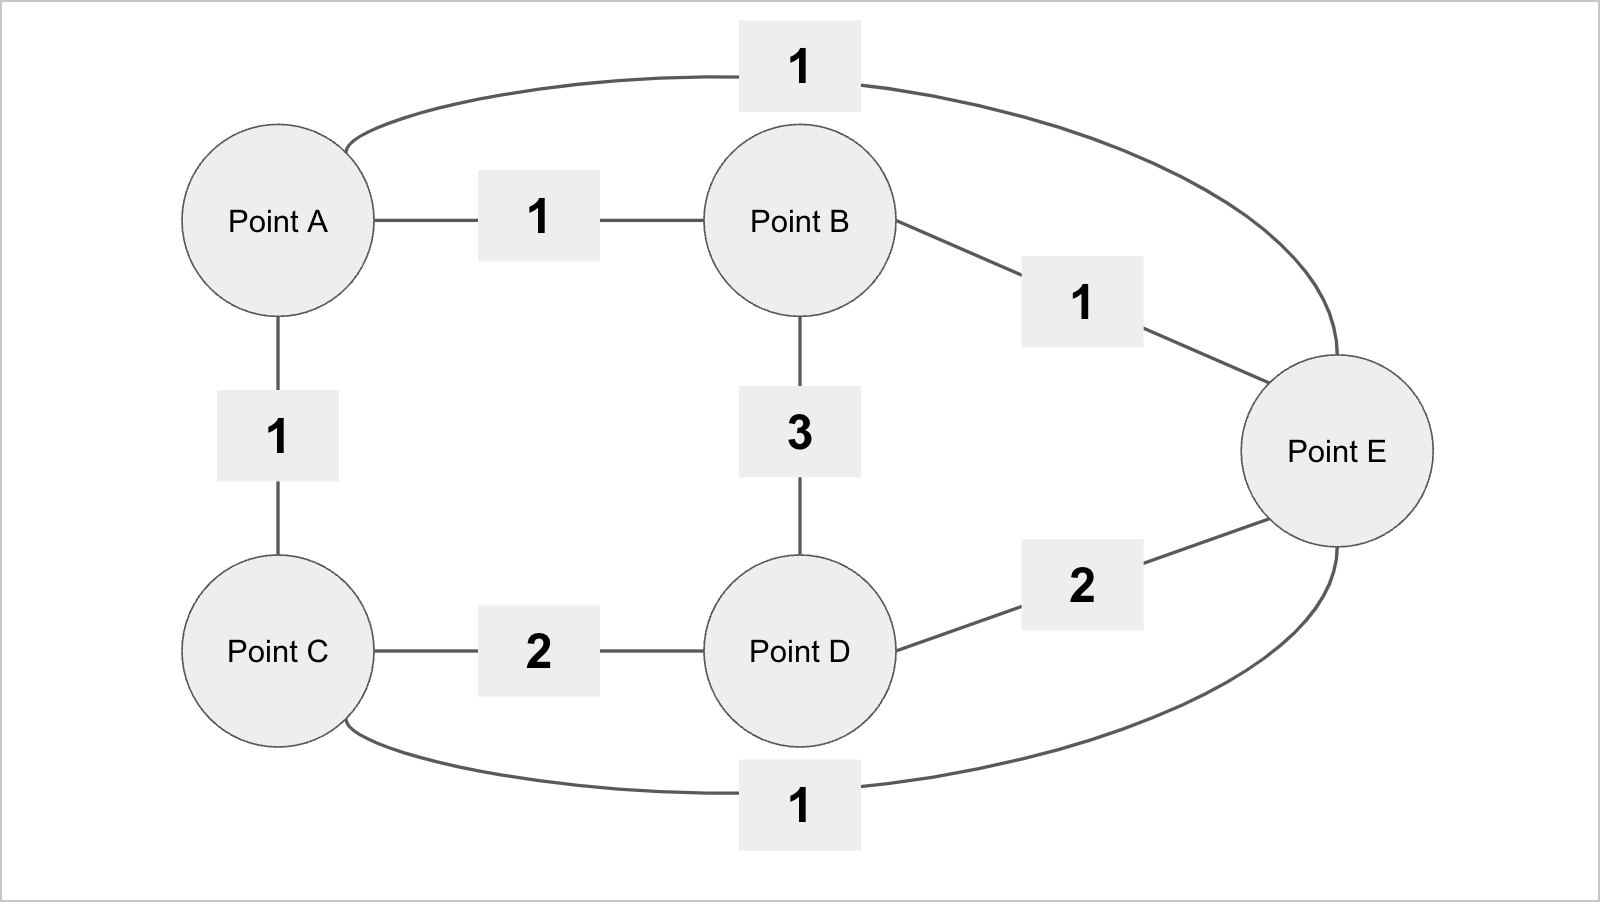
\includegraphics[width=4cm]{./image/03-Tech/chap3/sample_node.png}

\section{ディレクトリ構造}
\begin{tcolorbox}[breakable]
    \begin{verbatim}
├── build
│   ├── Docker
│   │   ├── go
│   │   │   └── Dockerfile
│   │   └── neo4j
│   │       ├── Dockerfile
│   │       └── volumes
│   │           ├── import
│   │           │   ├── done
│   │           │   ├── points.csv
│   │           │   └── route.csv
│   │           └── script
│   │               └── import_data.sh
│   └── docker-compose.yml
└── server
    ├── config
    │   ├── config.go
    │   └── environments
    │       └── neo4j.yml
    ├── controllers
    │   └── coordinate_controller.go
    ├── db
    │   └── neo4j.go
    ├── go.mod
    ├── go.sum
    ├── main.go
    ├── models
    │   └── coordinate.go
    ├── router
    │   └── router.go
    └── sample.http
\end{verbatim}
\end{tcolorbox}

\section{Neo4jに最初にインポートするファイル}
point.csv
\begin{tcolorbox}[breakable]
    \begin{verbatim}
1 point_id:ID,point_name,:LABEL
2 a,PointA,Point;Position
3 b,PointB,Point;Position
4 c,PointC,Point;Position
5 d,PointD,Point;Position
6 e,PointE,Point;Position
\end{verbatim}
\end{tcolorbox}

route.csv
\begin{tcolorbox}[breakable]
    \begin{verbatim}
:START_ID,:END_ID,:TYPE,cost:int
b,a,Distance,1
c,b,Distance,3
d,c,Distance,2
e,d,Distance,2
c,a,Distance,1
d,a,Distance,2
e,b,Distance,1
e,a,Distance,1
c,e,Distance,1
d,b,Distance,3
a,b,Distance,1
b,c,Distance,3
c,d,Distance,2
d,e,Distance,2
a,c,Distance,1
a,d,Distance,2
b,e,Distance,1
a,e,Distance,1
e,c,Distance,1
b,d,Distance,3
\end{verbatim}
\end{tcolorbox}
これらをNeo4jにインポートすることで、先ほどの図を表現することができます。
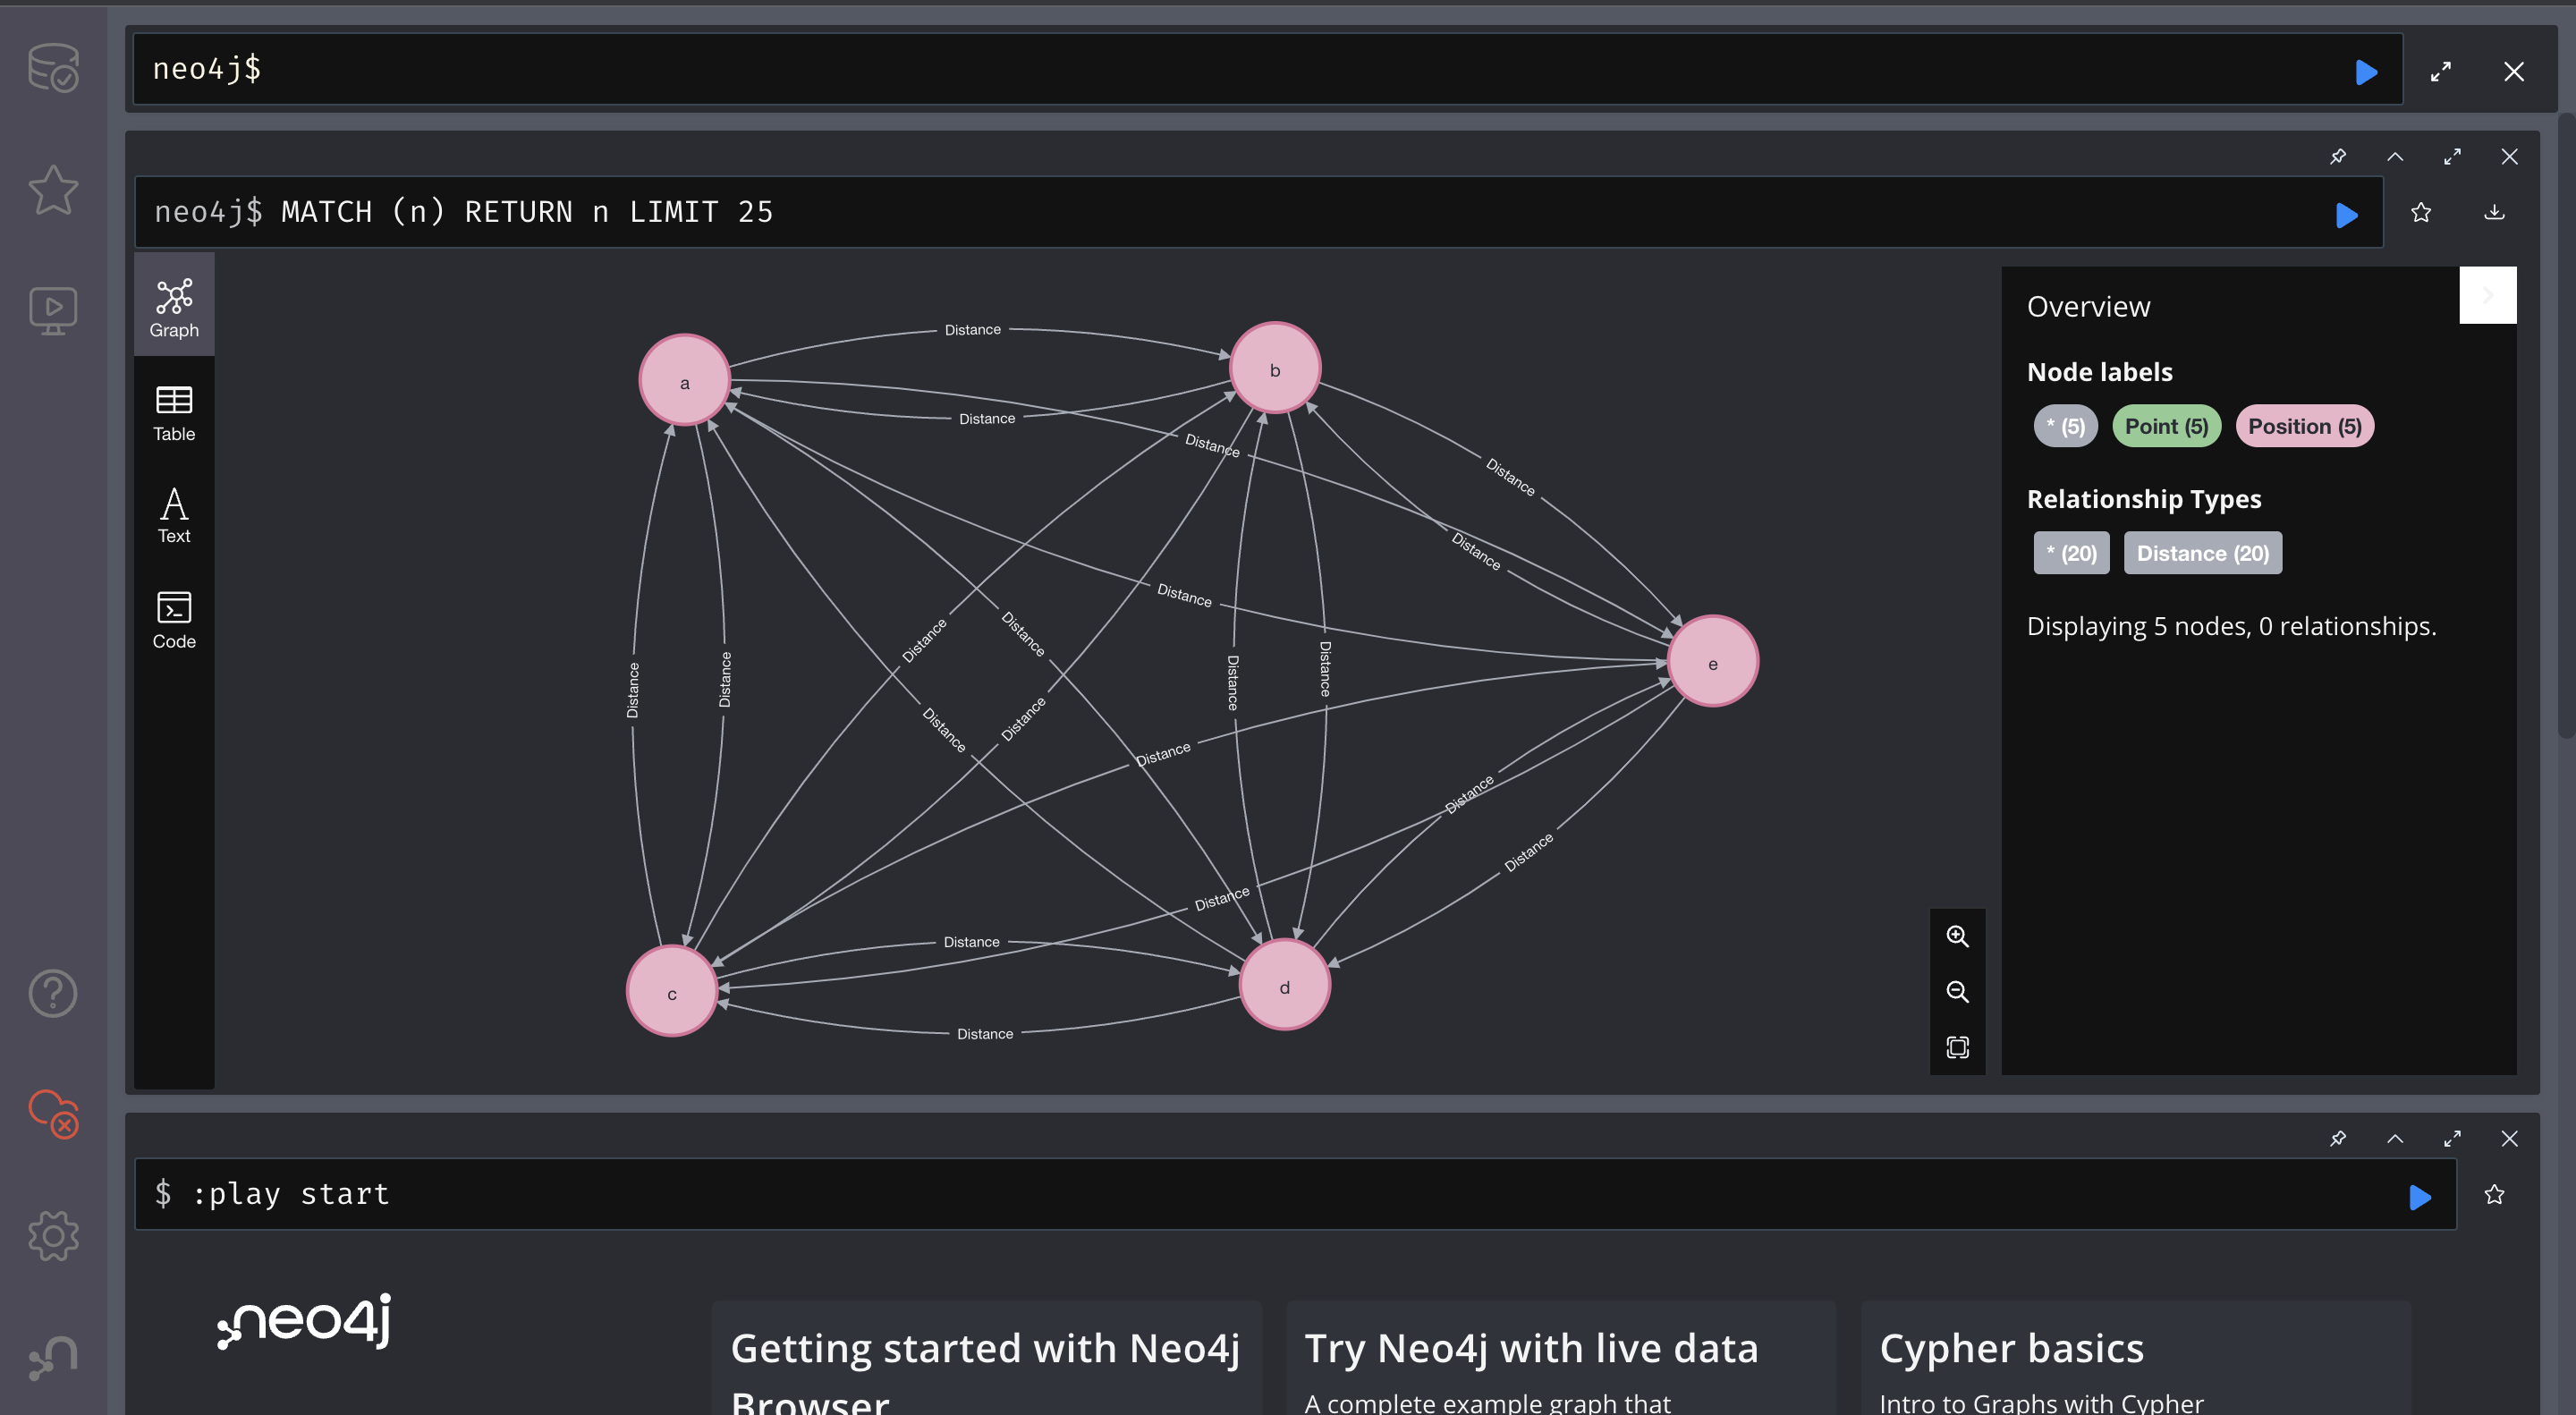
\includegraphics[width=4cm]{./image/03-Tech/chap3/neo4j_result.png}
無事できてますね。

\subsection{Docker環境の設定}
\begin{tcolorbox}[title=compose.yaml]
  \begin{verbatim}
```
    \begin{verbatim}
1 version: "3"
2 services:
3   go:
4     container_name: NEO4JAPI_GO
5     build:
6       context: ./docker/go
7       dockerfile: Dockerfile
8     stdin_open: true
9     tty: true
10    volumes:
11      - ../server:/server
12    ports:
13      - 8080:8080
14    networks:
15      app_net:
16        ipv4_address: 192.168.0.1
17    depends_on:
18      - "neo4j"
19
20  neo4j:
21    container_name: NEO4JAPI_NEO4J
22    build:
23      context: ./Docker/neo4j
24      dockerfile: Dockerfile
25    restart: always
26    ports:
27      - 57474:7474
28      - 57687:7687
29    volumes:
30      - ./Docker/neo4j/volumes/data:/data
31      - ./Docker/neo4j/volumes/logs:/logs
32      - ./Docker/neo4j/volumes/conf:/conf
33      - ./Docker/neo4j/volumes/import:/import
34      - ./Docker/neo4j/volumes/script:/script
35    environment:
36      - NEO4J_AUTH=neo4j/admin
37      - EXTENSION_SCRIPT=/script/import_data.sh
38    networks:
39      app_net:
40        ipv4_address: 192.168.0.2
41
42 networks:
43  app_net:
44    driver: bridge
45    ipam:
46      driver: default
47      config:
48        - subnet: 192.168.0.0/24
\end{verbatim}
\end{tcolorbox}
volumesはデータベースに入れるデータ、ログをバインドするための場所を指定しています。
environmentではユーザーとパスワード、最初に読み込んでもらうシェルスクリプトの場所を指定します。

go関連のDockerfile
\begin{tcolorbox}[breakable]
\begin{verbatim}
1  # goバージョン
2  FROM golang:1.19.3-alpine
3  # アップデートとgitのインストール
4  RUN apk add --update &&  apk add git
5  # appディレクトリの作成
6  RUN mkdir /server
7  # ワーキングディレクトリの設定
8  WORKDIR /server
9  # ホストのファイルをコンテナの作業ディレクトリに移行
10 ADD . /server
11 # main.goを実行
12 CMD ["go", "run", "main.go"]
\end{verbatim}
\end{tcolorbox}

Neo4j関連のDockerfile
\begin{tcolorbox}[title=dockerfile]
  \begin{verbatim}
```
\begin{verbatim}
1  # goバージョン
2  FROM golang:1.19.3-alpine
3  # アップデートとgitのインストール
4  RUN apk add --update &&  apk add git
5  # appディレクトリの作成
6  RUN mkdir /server
7  # ワーキングディレクトリの設定
8  WORKDIR /server
9  # ホストのファイルをコンテナの作業ディレクトリに移行
10 ADD . /server
11 # main.goを実行
12 CMD ["go", "run", "main.go"]
\end{verbatim}
\end{tcolorbox}

csvファイルを読ませるためのシェルスクリプト
\begin{tcolorbox}[breakable]
\begin{verbatim}
1  #!/bin/bash
2  set -euC
3
4  # EXTENSION_SCRIPTはコンテナが起動するたびにコールされるため、
5  # import処理が実施済かフラグファイルの有無をチェック
6  if [ -f /import/done ]; then
7      echo "Skip import process"
8      return
9  fi
10
11 # データを全削除
12 echo "delete database started."
13 rm -rf /data/databases
14 rm -rf /data/transactions
15 echo "delete database finished."
16
17 # CSVデータのインポート
18 echo "Start the data import process"
19 neo4j-admin import \
20   --nodes=/import/points.csv \
21   --relationships=/import/route.csv
22 echo "Complete the data import process"
23
24 # import処理の完了フラグファイルの作成
25 echo "Start creating flag file"
26 touch /import/done
27 echo "Complete creating flag file"
\end{verbatim}
\end{tcolorbox}
    
\section{Goのソースコード}
\subsection{configディレクトリ}
config.go
\begin{tcolorbox}[breakable]
\begin{verbatim}
1  package config
2
3  import (
4  	  "github.com/spf13/viper"
5  )
6
7  var n *viper.Viper
8
9  func init() {
10 	 n = viper.New()
11	 n.SetConfigType("yaml")
12 	 n.SetConfigName("neo4j")
13 	 n.AddConfigPath("config/environments/")
14 }
15
16 func GetNeo4jConfig() *viper.Viper {
17	 if err := n.ReadInConfig(); err != nil {
18		 return nil
19	 }
20	 return n
21 }
\end{verbatim}
\end{tcolorbox}
このファイルでneo4j.yamlの環境変数を読み込みます。
\begin{tcolorbox}[breakable]
\begin{verbatim}
1 neo4j:
2  user: neo4j
3  password: admin
4  uri: neo4j://192.168.176.1:57687
\end{verbatim}
\end{tcolorbox}
Neo4jと接続するための環境変数です。
\subsection{dbディレクトリ}
neo4j.go
\begin{tcolorbox}[breakable]
\begin{verbatim}
1  package db
2
3  import (
4	  "log"
5
6	  "neo4japi/server/config"
7
8	  "github.com/neo4j/neo4j-go-driver/v4/neo4j"
9  )
10
11 func GetDriverAndSession() neo4j.Session {
12	 n := config.GetNeo4jConfig()
13	 dr, err := neo4j.NewDriver(n.GetString("neo4j.uri"), neo4j.BasicAuth(n.GetString("neo4j.user"), n.GetString("neo4j.password"), ""))
14	 if err != nil {
15		 log.Fatal(err)
16	 }
17	 ses := dr.NewSession(neo4j.SessionConfig{AccessMode: neo4j.AccessModeRead})
18	 return ses
19 }
20
\end{verbatim}
\end{tcolorbox}
このファイルでNeo4jと接続し、セッションを返すようにします。
\subsection{modelsディレクトリ}
coordinate.go
\begin{tcolorbox}[breakable]
\begin{verbatim}
1  package models
2
3  import (
4	  "fmt"
5	  "log"
6
7	  "neo4japi/server/db"
8
9	  "github.com/neo4j/neo4j-go-driver/v4/neo4j"
10 )
11
12 type Route struct {
13	 Position string `json:"point"`
14 }
15
16 func FindRoute(fr, to string) []*Route {
17 	 var r []*Route
18	 ses := db.GetDriverAndSession()
19	 defer ses.Close()
20	 cyp := fmt.Sprintf(`
21		 MATCH (from:Position {point_name: "%s"}), (to:Position {point_name: "%s"}), 
22			 path=allShortestPaths ((from)-[distance:Distance*]->(to))
23		 WITH
24			 [position in nodes(path) | position.point_name] as name,
25		 REDUCE(totalMinutes = 0, d in distance | totalMinutes + d.cost) as 所要時間
26		 RETURN name
27		 ORDER BY 所要時間
28		 LIMIT 10;
29	 `, fr, to)
30
31	 _, err := ses.ReadTransaction(func(transaction neo4j.Transaction) (interface{}, error) {
32		 result, err := transaction.Run(cyp, nil)
33		 if err != nil {
34			 return nil, err
35		 }
36		 if result.Next() {
37			 name, _ := result.Record().Get("name")
38			 nameAr := name.([]interface{})
39
40			 for i := 0; i < len(nameAr); i++ {
41				 r = append(r, &Route{nameAr[i].(string)})
42			 }
43		 }
44		 return nil, result.Err()
45	 })
46	 if err != nil {
47		 log.Fatal(err)
48	 }
49	 return r
50 }
\end{verbatim}
\end{tcolorbox}

出発地点と目的地を受け取ることでNeo4jにCypherというクエリ言語を用いて最短経路を導出してもらいます。
\subsection{controllersディレクトリ}
coordinate\_controller.go
\begin{tcolorbox}[breakable]
\begin{verbatim}
1  package controllers
2
3  import (
4	  "net/http"
5
6	  "github.com/gin-gonic/gin"
7	  "neo4japi/server/models"
8  )
9
10 func RouteSearch(c *gin.Context) {
11	 fr := c.Query("fr")
12	 to := c.Query("to")
13	 res := models.FindRoute(fr, to)
14	 c.JSON(http.StatusOK, res)
15 }
\end{verbatim}
\end{tcolorbox}
GETリクエストで受け取ったパラメータを models で作成した関数に渡します。
\subsection{routerディレクトリ}
router.go
\begin{tcolorbox}[breakable]
\begin{verbatim}
1  package router
2
3  import (
4	  "github.com/gin-gonic/gin"
5	  "neo4japi/server/controllers"
6  )
7
8  func Init() {
9	  r := gin.Default()
10	 r.GET("/coordinate", controllers.RouteSearch)
11	 r.Run()
12 }
\end{verbatim}
\end{tcolorbox}
ルーティング先を定義します。
\subsection{実行ファイル}
coordinate\_controller.go
\begin{tcolorbox}[breakable]
\begin{verbatim}
1  package main
2
3  import (
4	  "neo4japi/server/router"
5  )
6
7  func main() {
8	  router.Init()
9  }
\end{verbatim}
\end{tcolorbox}

\section{実行方法}
\begin{tcolorbox}[breakable]
\begin{verbatim}
docker compose up
\end{verbatim}
\end{tcolorbox}
このコマンドを実行することで Neo4j サーバーと Gin サーバーが立ち上がります。
\subsection{実行確認}
sample.http
\begin{tcolorbox}[breakable]
\begin{verbatim}
1  GET http://localhost:8080/coordinate?fr=PointB&to=PointE
\end{verbatim}
\end{tcolorbox}
% ここで、 coordinate?fr=PointB&to=PointE の部分を自分の好きな地点にしてリクエストを送ると、最短経路が返されます。

\lstdefinelanguage{JavaScript}{
  keywords={const, let, var, export, default, function, return, if, else, while, for, switch, case, break, throw, catch, typeof, instanceof, import},
  keywordstyle=\color{blue}\bfseries,
  ndkeywords={class, export, boolean, throw, implements, import, this},
  ndkeywordstyle=\color{darkgray}\bfseries,
  identifierstyle=\color{black},
  sensitive=false,
  comment=[l]{//},
  morecomment=[s]{/*}{*/},
  commentstyle=\color{purple}\ttfamily,
  stringstyle=\color{red}\ttfamily,
  morestring=[b]',
  morestring=[b]",
}

\lstdefinelanguage{TypeScript}{
  keywords={const, let, var, export, default, function, return, if, else, while, for, switch, case, break, throw, catch, typeof, instanceof, import, as, type, keyof, typeof, this},
  keywordstyle=\color{blue}\bfseries,
  ndkeywords={class, interface, enum, extends, implements, readonly, abstract, static, public, private, protected, any, boolean, number, string, object, unknown, null, void, never},
  ndkeywordstyle=\color{darkgray}\bfseries,
  identifierstyle=\color{black},
  sensitive=false,
  comment=[l]{//},
  morecomment=[s]{/*}{*/},
  commentstyle=\color{purple}\ttfamily,
  stringstyle=\color{red}\ttfamily,
  morestring=[b]',
  morestring=[b]",
}

\lstdefinestyle{customstyle}{
  language=TypeScript,
  basicstyle=\ttfamily,
  breaklines=true,
  breakatwhitespace=false,
  columns=fullflexible,
  keepspaces=true,
}



\chapter{Next.js 13 触ってみた}
\section{はじめに}
10 月後半に行われた Next.js Conf 2022 で発表された Next.js 13 を実際に触って
みたのでその内容を書きます。当初は全体を網羅して書く予定だったのですが量が多
かったの少し絞ってます。対象読者としてある程度 React や Next.js を触っている
人を対象としています。


\section{プロジェクト作成からサーバ起動}

TypeScriptとESLintを入れるか聞かれるので入れる。
\begin{tcblisting}{listing only, breakable}
  $ npx create-next-app@latest --ts
\end{tcblisting}



pagesディレクトリを削除。
\begin{tcblisting}{listing only, breakable}
  $ rm -rf pages
\end{tcblisting}





appディレクトリを作る。
\begin{tcblisting}{listing only, breakable}
  $ mkdir app
\end{tcblisting}


appディレクトリは実験段階の機能なので,next.config.jsを変更する。

\begin{tcblisting}{title={next.config.js},listing options={style=customstyle},listing only, breakable}
  const nextConfig = {
  reactStrictMode: true,
  swcMinify: true,
  experimental: {
    appDir: true,
  },
};
\end{tcblisting}

app/page.tsxを作り、以下のようにする。



\begin{tcblisting}{title={app/page.tsx},listing only, breakable}
  export default function Page() {
      return <h1>Hello, Next.js!</h1>;
    }
\end{tcblisting}




ローカルサーバ起動。


\begin{tcblisting}{listing only, breakable}
  $ npm run dev
\end{tcblisting}



ブラウザで http://localhost:3000/ にアクセスすると、Hello, Next.js! が表示される。

\begin{figure}[H]
  \centering
  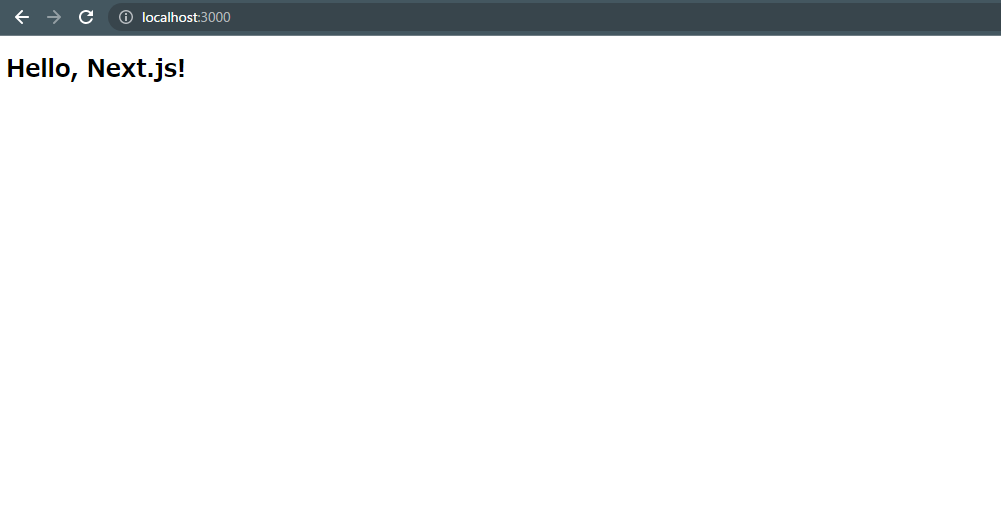
\includegraphics[width=12cm]{./image/03-Tech/chap4/01.png}
  \caption{Hello,Next.js}

\end{figure}




\section{LayoutとHead}

サーバを起動すると自動的にappディレクトリにlayout.tsx、head.tsxというファイルが作られていました。

next/headを使って各ページファイルにheadを定義していたのがhead.tsxに書けるようになったみたいですね。

\begin{tcblisting}{title={head.tsx},listing options={style=customstyle},listing only, breakable}
  export default function Head() {
      return (
      <>
        <title></title>
        <meta content="width=device-width, initial-scale=1" name="viewport" />
        <link rel="icon" href="/favicon.ico" />
      </>
      )
    }
\end{tcblisting}



ページの共通レイアウトを定義するファイル。




\begin{tcblisting}{listing options={style=customstyle},listing only, breakable}
  export default function RootLayout({
      children,
    }: {
  children: React.ReactNode
  }) {
      return (
      <html>
        <head />
        <body>{children}</body>
      </html>
      )
    }

\end{tcblisting}


今までは\_app.tsxなどに下記のようにレイアウトを定義していました。
\begin{tcblisting}{title={\_app.tsx},listing options={style=customstyle},listing only, breakable}
  <Layout>
    <Component {...pageProps} />
  </Layout>
\end{tcblisting}




この方法だとページごとにレイアウトを変えられないです。
なのでページごとにレイアウトを変えたい場合はgetLayoutを用いる必要がありました。
Next.js 13ではレイアウトを変えたいページがあるディレクトリにlayout.tsxを置けばページごとにレイアウトを変えられるようになりました。


ここではダッシュボードページのレイアウトの場合を考えます。
appディレクトリの中でdashbordディレクトリを作成して以下のようにlayout.tsxを配置するだけです。



\begin{tcblisting}{title={
        app/dashboard/layout.tsx
      },listing options={style=customstyle},listing only, breakable}
  export default function DashboardLayout({
      children,
    }: {
  children: React.ReactNode;
  }) {
      return <section>{children}</section>;
    }

\end{tcblisting}




少し疑問に思ったのがdashboardディレクトリのpage.tsxではRootLayoutは呼ばれずDashboardLayoutのみが呼ばれるのかと思っていました。しかし、実際には入れ子構造で呼び出されるようです。

公式の画像がわかりやすいので貼っておきます。
\begin{figure}[H]
  \centering
  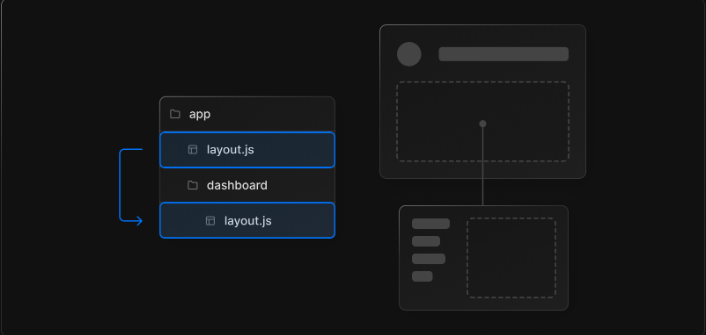
\includegraphics[width=12cm]{./image/03-Tech/chap4/02.png}
  \caption{layout.jsの適用範囲}
\end{figure}

次の機能に行く前にdashboardディレクトリにpage.tsxも作っておきます。
\begin{tcblisting}{title={
        app/dashboard/layout.tsx
      },listing options={style=customstyle},listing only, breakable}
  export default function DashBoardPage() {
      return <h1>DashBoard Page</h1>;
  }

\end{tcblisting}


違いがわかりやすいように他のファイルも変更します。
\begin{tcblisting}{title={
        app/layout.tsx
      },listing options={style=customstyle},listing only, breakable}
      export default function RootLayout({
        children,
      }: {
        children: React.ReactNode;
      }) {
        return (
          <html>
            <head />
            <body
              style={{
                backgroundColor: '#C0C0C0',
                padding: '50px',
              }}
            >
              {children}
            </body>
          </html>
        );
      }
      

\end{tcblisting}




\begin{tcblisting}{title={
        app/dashboard/layout.tsx
      },listing options={style=customstyle},listing only, breakable}
      export default function DashboardLayout({
        children,
      }: {
        children: React.ReactNode;
      }) {
        return (
          <section
            style={{
              backgroundColor: 'white',            
            }}
          >
            {children}
          </section>
        );
      }
\end{tcblisting}



ページの見た目が画像のようになってればOK。


\begin{figure}[H]
  \centering
  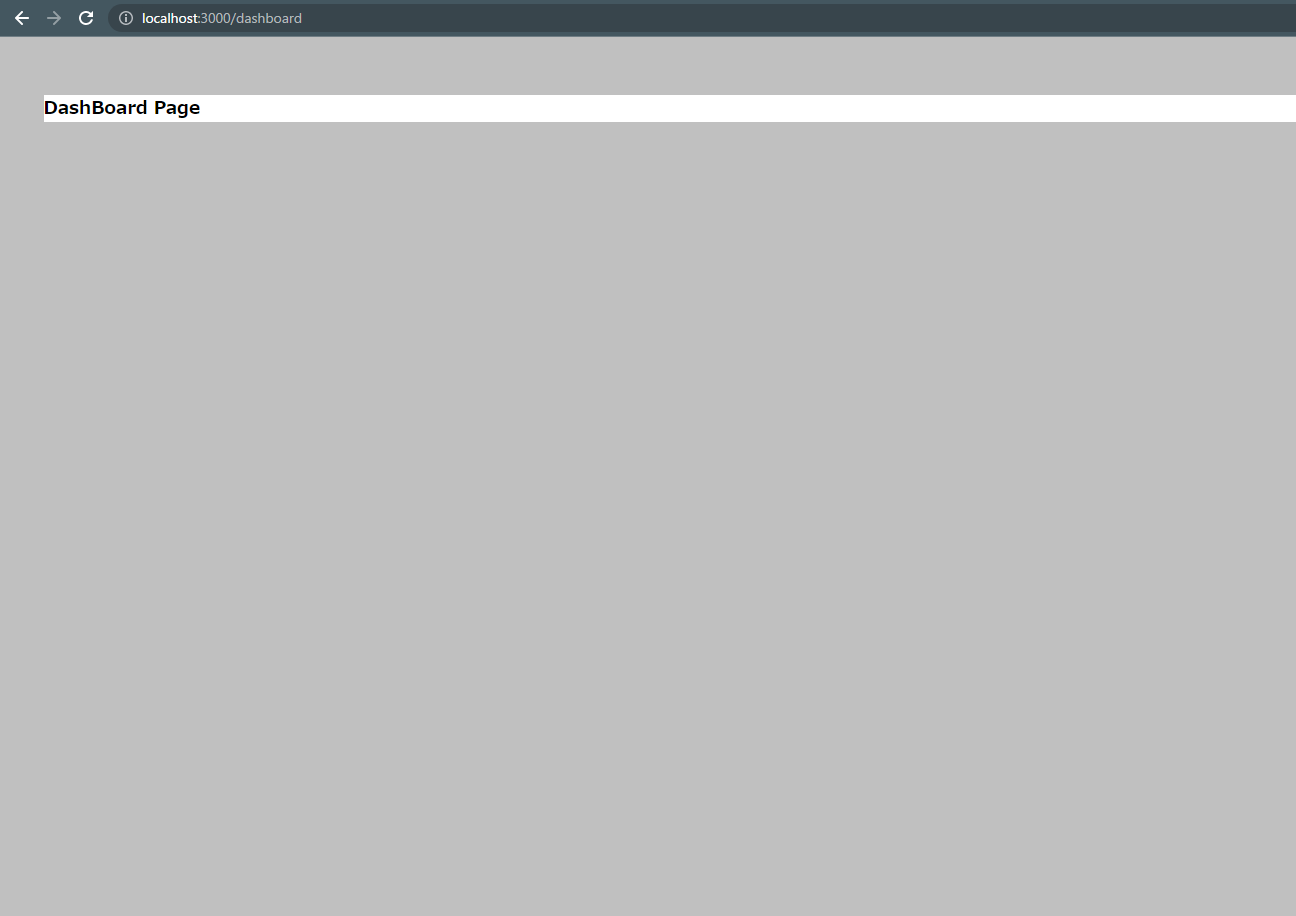
\includegraphics[width=12cm]{./image/03-Tech/chap4/03.png}
  \caption{DashBoardページ}
\end{figure}










\section{React Server Components}
React Server Components(RSC)はReact18で追加された機能でクライアントと
サーバ側が協調してアプリケーションをレンダリングできる機能です。
これによりコンポーネントごとに最適なレンダリング方法を選択できるようになります。
例えばデータの取得はサーバ側で行い,ユーザの操作によって変わる部分はクライアント側で
レンダリングできます。これも公式ドキュメントの図がわかりやすいので貼っておきます。


\begin{figure}[H]
  \centering
  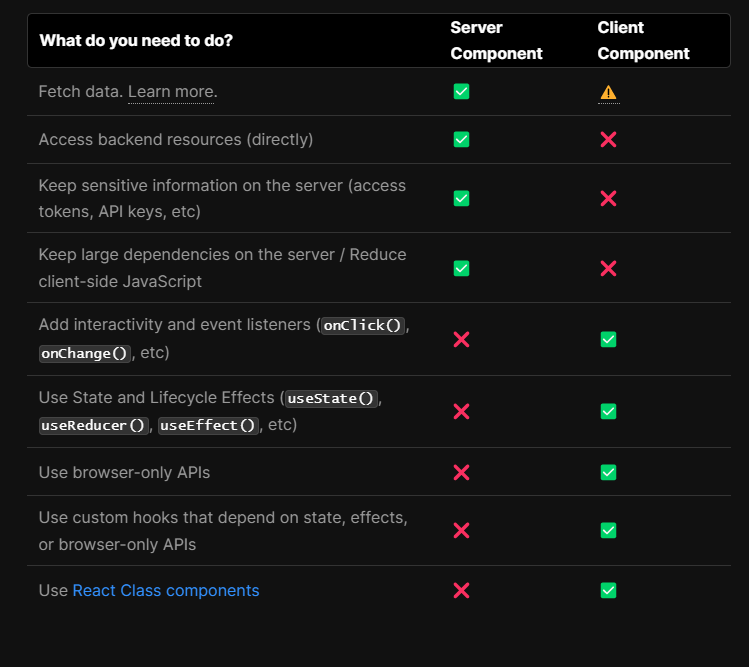
\includegraphics[width=12cm]{./image/03-Tech/chap4/04.png}
  \caption{Sever ComponentとClient Componentsの違い}
\end{figure}



またSSRとの違いとしてクライアント側のJavaScriptの量を減らせる点です。
SSRの場合ハイドレーション(サーバ側で生成したDOMとクライアントで生成したDOMを合成する)というステップがありページを早く表示できてもクライアント側でも同じ処理が走るためJavaScriptの量は同じでした。
RSCはサーバ側でレンダリングした後残りをクライアント側でレンダリングします.これによってクライアント側に送信されるJavaScriptの量を減らせます。


\section{サーバーコンポーネントでデータを取得}


appディレクトリ内のコンポーネントはデフォルトだとサーバコンポーネントになっています。
以下のコードはサーバサイドでqiitaの記事リスト取得して表示するものです。
dashboard/page.tsxを書き換えます。



\begin{tcblisting}{title={
        dashboard/page.tsx
      },listing options={style=customstyle},listing only, breakable}
  type Article = {
    id: number;
    title: string;
  };

  async function getArticle(): Promise<Article[]> {
    const res = await fetch('https://qiita.com/api/v2/items?page=1&per_page=24');

    if (!res.ok) {
        throw new Error('Failed to fetch data');
    }

    return res.json();
  }

  export default async function DashBoardPage() {
    const articles = await getArticle();

    return (
      <div>
        <h1>Dashboard</h1>
        <div
        style={{
            display: 'flex',
            flexDirection: 'column',
            flexWrap: 'wrap',
            height: '50vh',
          }}
        >
          {articles?.map((article) => (
            <div
            key={article.id}
            style={{
                display: 'flex',
                gap: '10px',
              }}
            >
              <p>{article.title}</p>
            </div>
            ))}
        </div>
      </div>
    );
  }


\end{tcblisting}






画像のように表示される。

\begin{figure}[H]
  \centering
  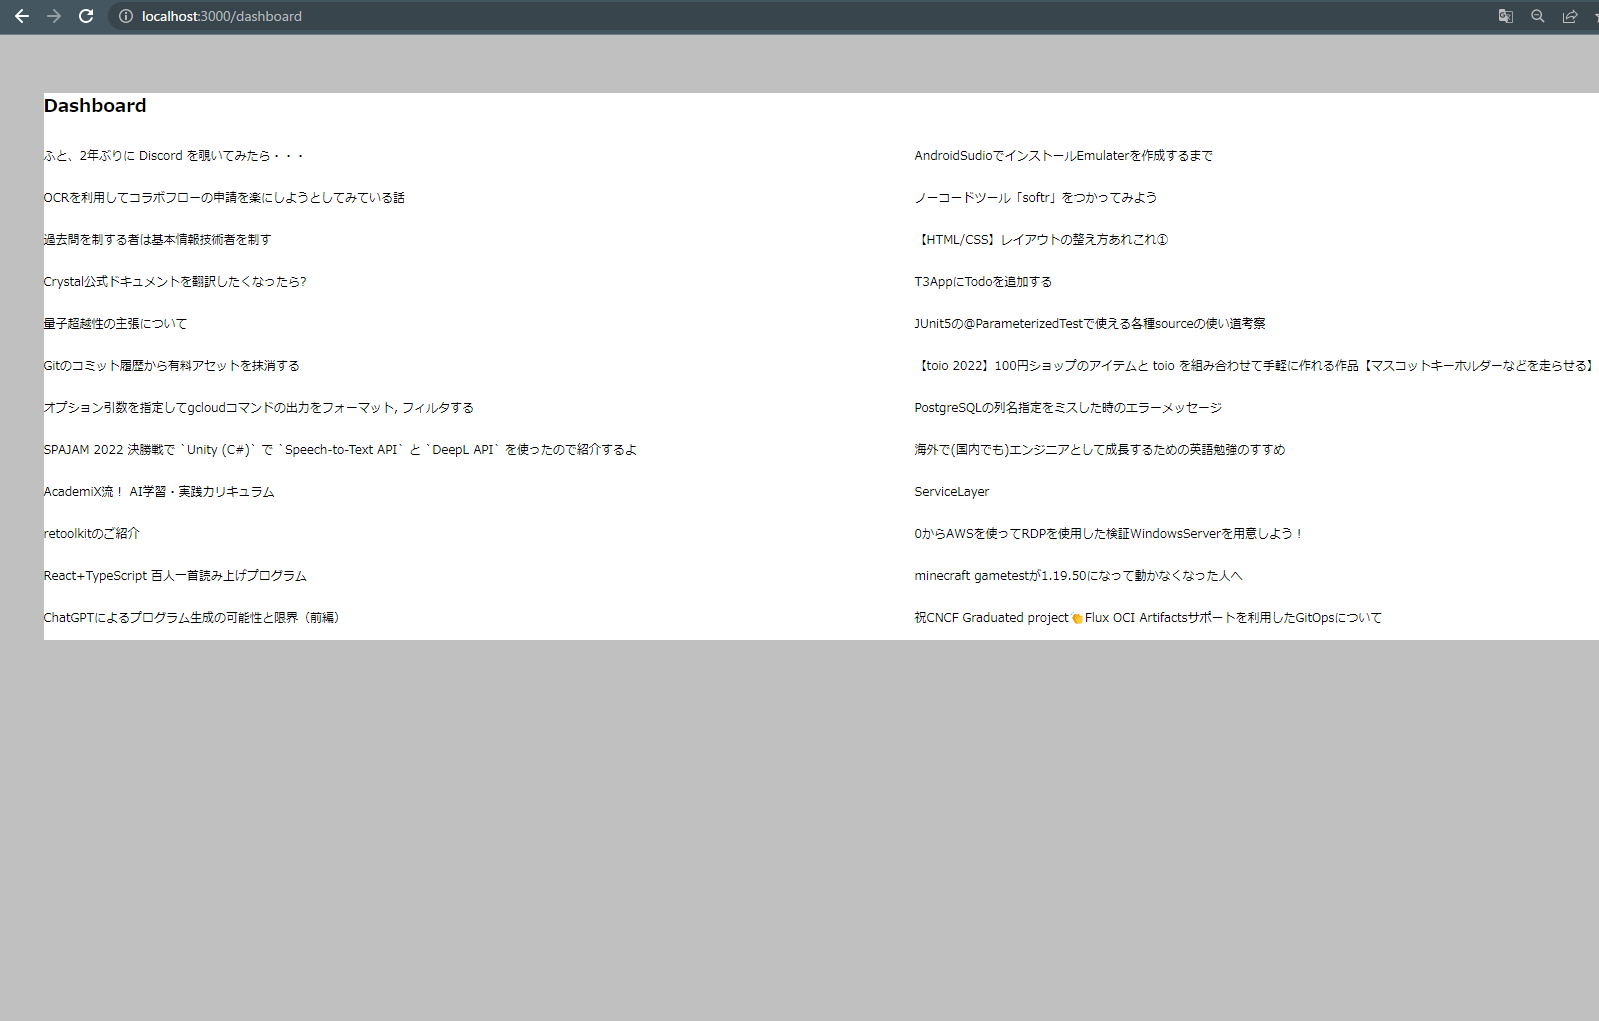
\includegraphics[width=12cm]{./image/03-Tech/chap4/06.png}
  \caption{APIからデータ取得後のページ}
\end{figure}


サイトにカーソルを合わせて右クリックしてページのソースを表示をクリックしてみましょう。
あらかじめデータが入った状態でサーバから送られてくるのでページソースに記事データが表示されています。

\begin{figure}[H]
  \centering
  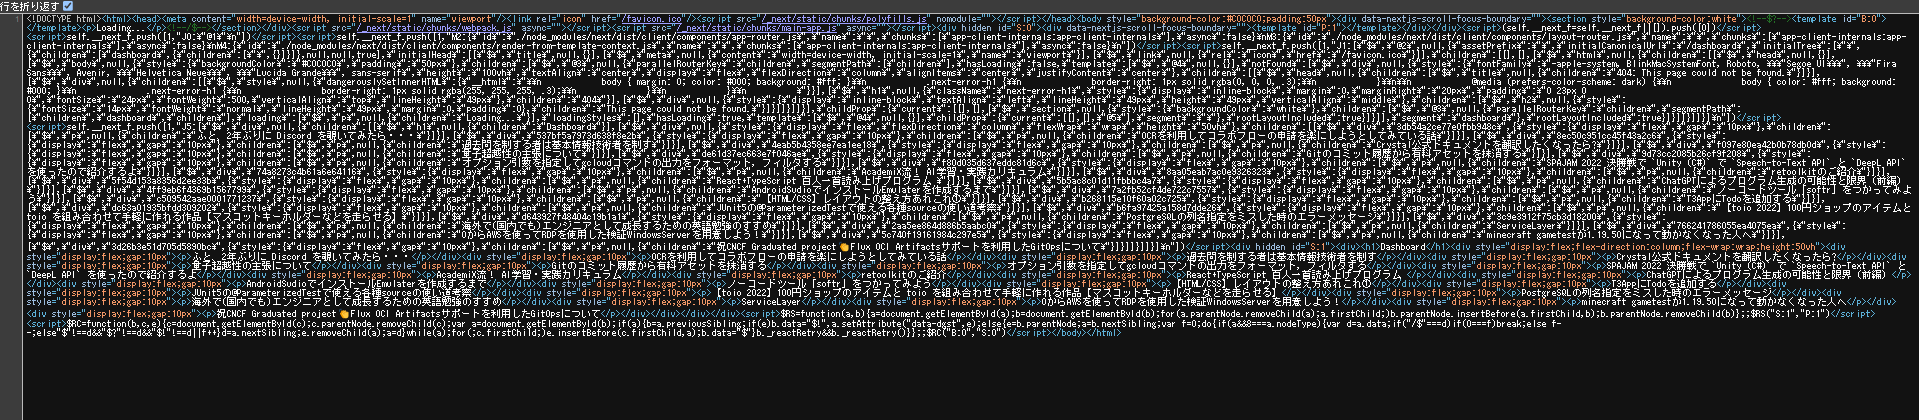
\includegraphics[width=12cm]{./image/03-Tech/chap4/05.png}
  \caption{ページのソース表示}
\end{figure}

\section{ローディングUI表示}

次はローディングUIを表示する機能です。
dashboradディレクトリにloading.tsxを作成します。

\begin{tcblisting}{title={
        loading.tsx
      },listing options={style=customstyle},listing only, breakable}
  export default function Loading() {
    return <p>Loading...</p>;
  }
\end{tcblisting}


データの取得が終わり、pageコンポーネントがレンダリングされるまでの間はLoadingコンポーネントが表示されます。

\begin{figure}[H]
  \centering
  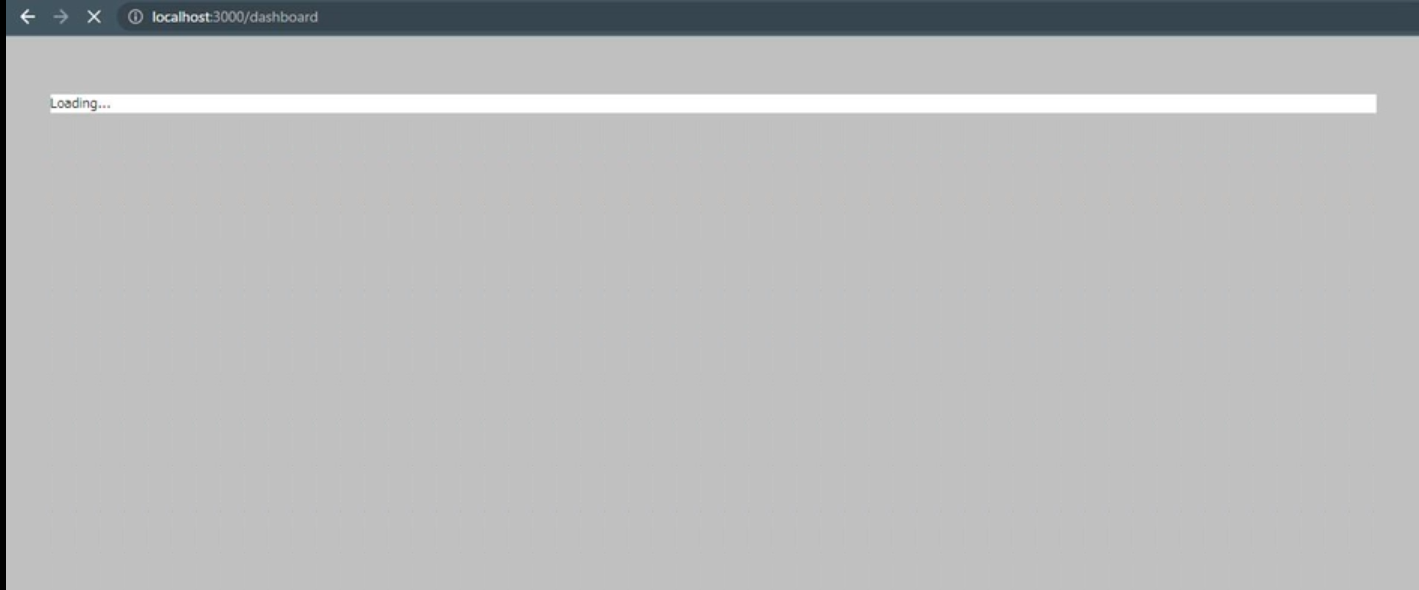
\includegraphics[width=12cm]{./image/03-Tech/chap4/07.png}
  \caption{ローディングUI}
\end{figure}




これはReact18で追加されたSuspenseという機能が使われていてます。
Suspenseについて説明するとコンポーネントが表示されるまでの状態を指定できるコンポーネントです。
非同期的なコンポーネントの場合レンダリングに時間がかかるためその間に何を表示させるかをSuspenseを使うと指定できるようになります。

具体的な使用例を上げます。下のコードはデータフェッチライブラリ React Queryを使ったデータ取得と表示のサンプルです。






\begin{tcblisting}{listing options={style=customstyle}, listing only, breakable}
  import { QueryClient, QueryClientProvider, useQuery } from 'react-query';

  const queryClient = new QueryClient();

  export default function App() {
    return (
    <QueryClientProvider client={queryClient}>
    <Example />
    </QueryClientProvider>
    );
  }
  export function Loading() {
      return <p>Loading...</p>;
  }

  function Example() {
    const { isLoading, data } = useQuery('repoData', () =>
    fetch('https://api.github.com/repos/tannerlinsley/react-query').then(
    (res) => res.json()
    )
    );

    if (isLoading) return <Loading />;

    return (
      <div>
        <h1>{data.name}</h1>
        <p>{data.description}</p>
      </div>
    );
  }
\end{tcblisting}




Suspenseを使えば下のコードに置き換えられます。


\begin{tcblisting}{listing options={style=customstyle},listing only, breakable}
import { Suspense } from 'react';
import { QueryClient, QueryClientProvider, useQuery } from 'react-query';

const queryClient = new QueryClient();

export default function App() {
  return (
    <QueryClientProvider client={queryClient}>
      {/* suspenseコンポーネントででラップ */}
      <Suspense fallback={<Loading />}>
        <Example />
      </Suspense>
    </QueryClientProvider>
  );
}
export function Loading() {
  return <p>Loading...</p>;
}

function Example() {
  const { data } = useQuery('repoData', () =>
    fetch('https://api.github.com/repos/tannerlinsley/react-query').then(
      (res) => res.json()
    )
  );
  //ローディングプロパティによる表示分岐の削除

  return (
    <div>
      <h1>{data.name}</h1>
      <p>{data.description}</p>
    </div>
  );
}

\end{tcblisting}





変更点はExampleコンポーネントをSuspenseコンポーネントでラップしているのと、Exampleコンポーネントの中のisLoadingプロパティを使った表示切替の部分が消えているところです。
Suspenseのいいところはデータ取得をするコンポーネントの中で表示を切り替える処理を書く必要がない所です。
これによってより宣言的なコードになりました。またコンポーネントの責務の観点から見てもローディング完了時の表示だけでよくシンプルになっています。

Next.js 13ではloading.tsxを置いてあげるとNext.js側がそれを読み取りPageコンポーネントをSuspenseコンポーネントでラップしてくれるようです。
普通に書くと以下のようになります。



\begin{tcblisting}{listing only, breakable}
  <Layout>
    <Headr/>
    <SideNav/>
    <Suspense fallback={<Loading />}>
      <DashBoardPage />
    </Suspense>
  </Layout>
\end{tcblisting}

ディレクトリ内にloading.tsxを配置すると、自動的にこのコードを記述した動作が実現されます。



\section{エラーハンドリング}

次にエラーハンドリングを見ていきます。
dashboardディレクトリにerror.tsxを作成します。


\begin{tcblisting}{title={
        dashboard/error.tsx
      },listing options={style=customstyle},listing only, breakable}
'use client';

import { useEffect } from 'react';

export default function Error({
  error,
  reset,
}: {
  error: Error;
  reset: () => void;
  }) {
  useEffect(() => {
  // Log the error to an error reporting service
  console.error(error);
  }, [error]);

  return (
  <div>
    <p>Something went wrong!</p>
    <button onClick={() => reset()}>Reset error boundary</button>
  </div>
  );
}
\end{tcblisting}



公式ドキュメントによるとerror.tsxはクライアントコンポーネントである必要がありuse client;と書けばクライアントコンポーネントして利用するできるようです。
loading.tsxと同じようにファイルを置いておけば自動的にPageをネストしてエラーハンドリングをしているようです。

普通に書いた場合


\begin{tcblisting}{title={
  dashboard/error.tsx
},listing options={style=customstyle},listing only, breakable}
<Layout>
    <Headr/>
    <SideNav/>
    <ErrorBoundary fallback={<Loading />}>
      <DashBoardPage />
    </ErrorBoundary>
</Layout>
\end{tcblisting}



ただこれを見てわかる通りpageをラップしてるので同階層のコンポーネントのエラーハンドリングはできない感じですね.したいならより上の階層でErrorBoundaryを使う必要がありそうです。

実際にコードを書き換えてエラーを出してみます。
存在しないURL'hoge'を指定しgetArticleでしていたエラーハンドリングを削除しています。


\begin{tcblisting}{title={

        dashboard/page.tsx
      },listing options={style=customstyle},listing only, breakable}

'use client';

import { useEffect } from 'react';
      
export default function Error({
  error,
  reset,
}: {
  error: Error;
  reset: () => void;
}) {
  useEffect(() => {
    // Log the error to an error reporting service
    console.error(error);
  }, [error]);
      
  return (
    <div>
      <p>Something went wrong!</p>
      <button onClick={() => reset()}>Reset error boundary</button>
    </div>
  );
}

\end{tcblisting}


エラーの内容とエラーページが表示されていますね。


\begin{figure}[H]
  \centering
  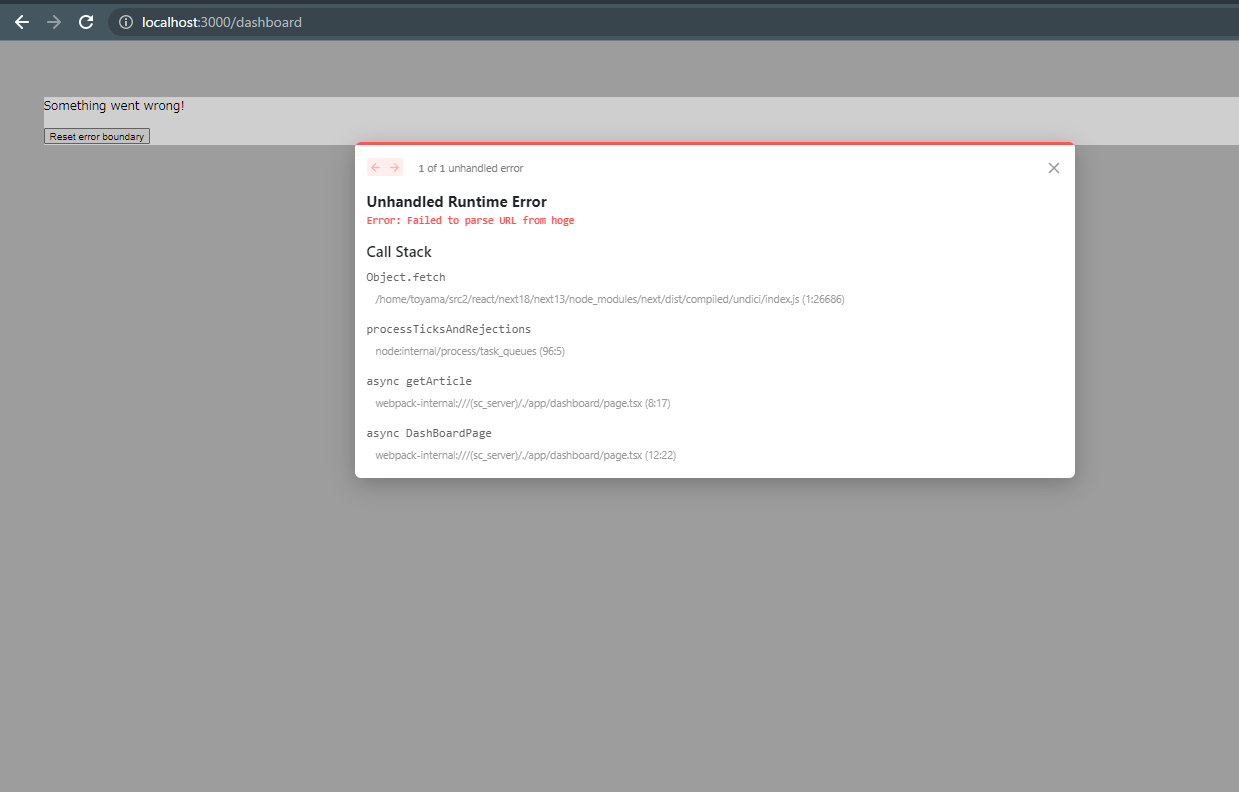
\includegraphics[width=12cm]{./image/03-Tech/chap4/08.png}
  \caption{エラーハンドリング画面}
\end{figure}



\section{終わりに}
感想としては、Next.js 13の機能はReact18のSupenseやRSCなどの機能に合わせたアップデートというのを強く感じました。
\chapter{シス研の日常}

シス研は技術一辺倒ではなく、次のような活動をしているメンバーもいます!

\begin{tcolorbox}[title=お品書き]
  \begin{itemize}
    \item p.47『戦闘機に乗ろう』松土
          戦闘機のフライトシュミレータの紹介をしています!
  \end{itemize} 
\end{tcolorbox}

\begin{figure}[H]
  \centering
  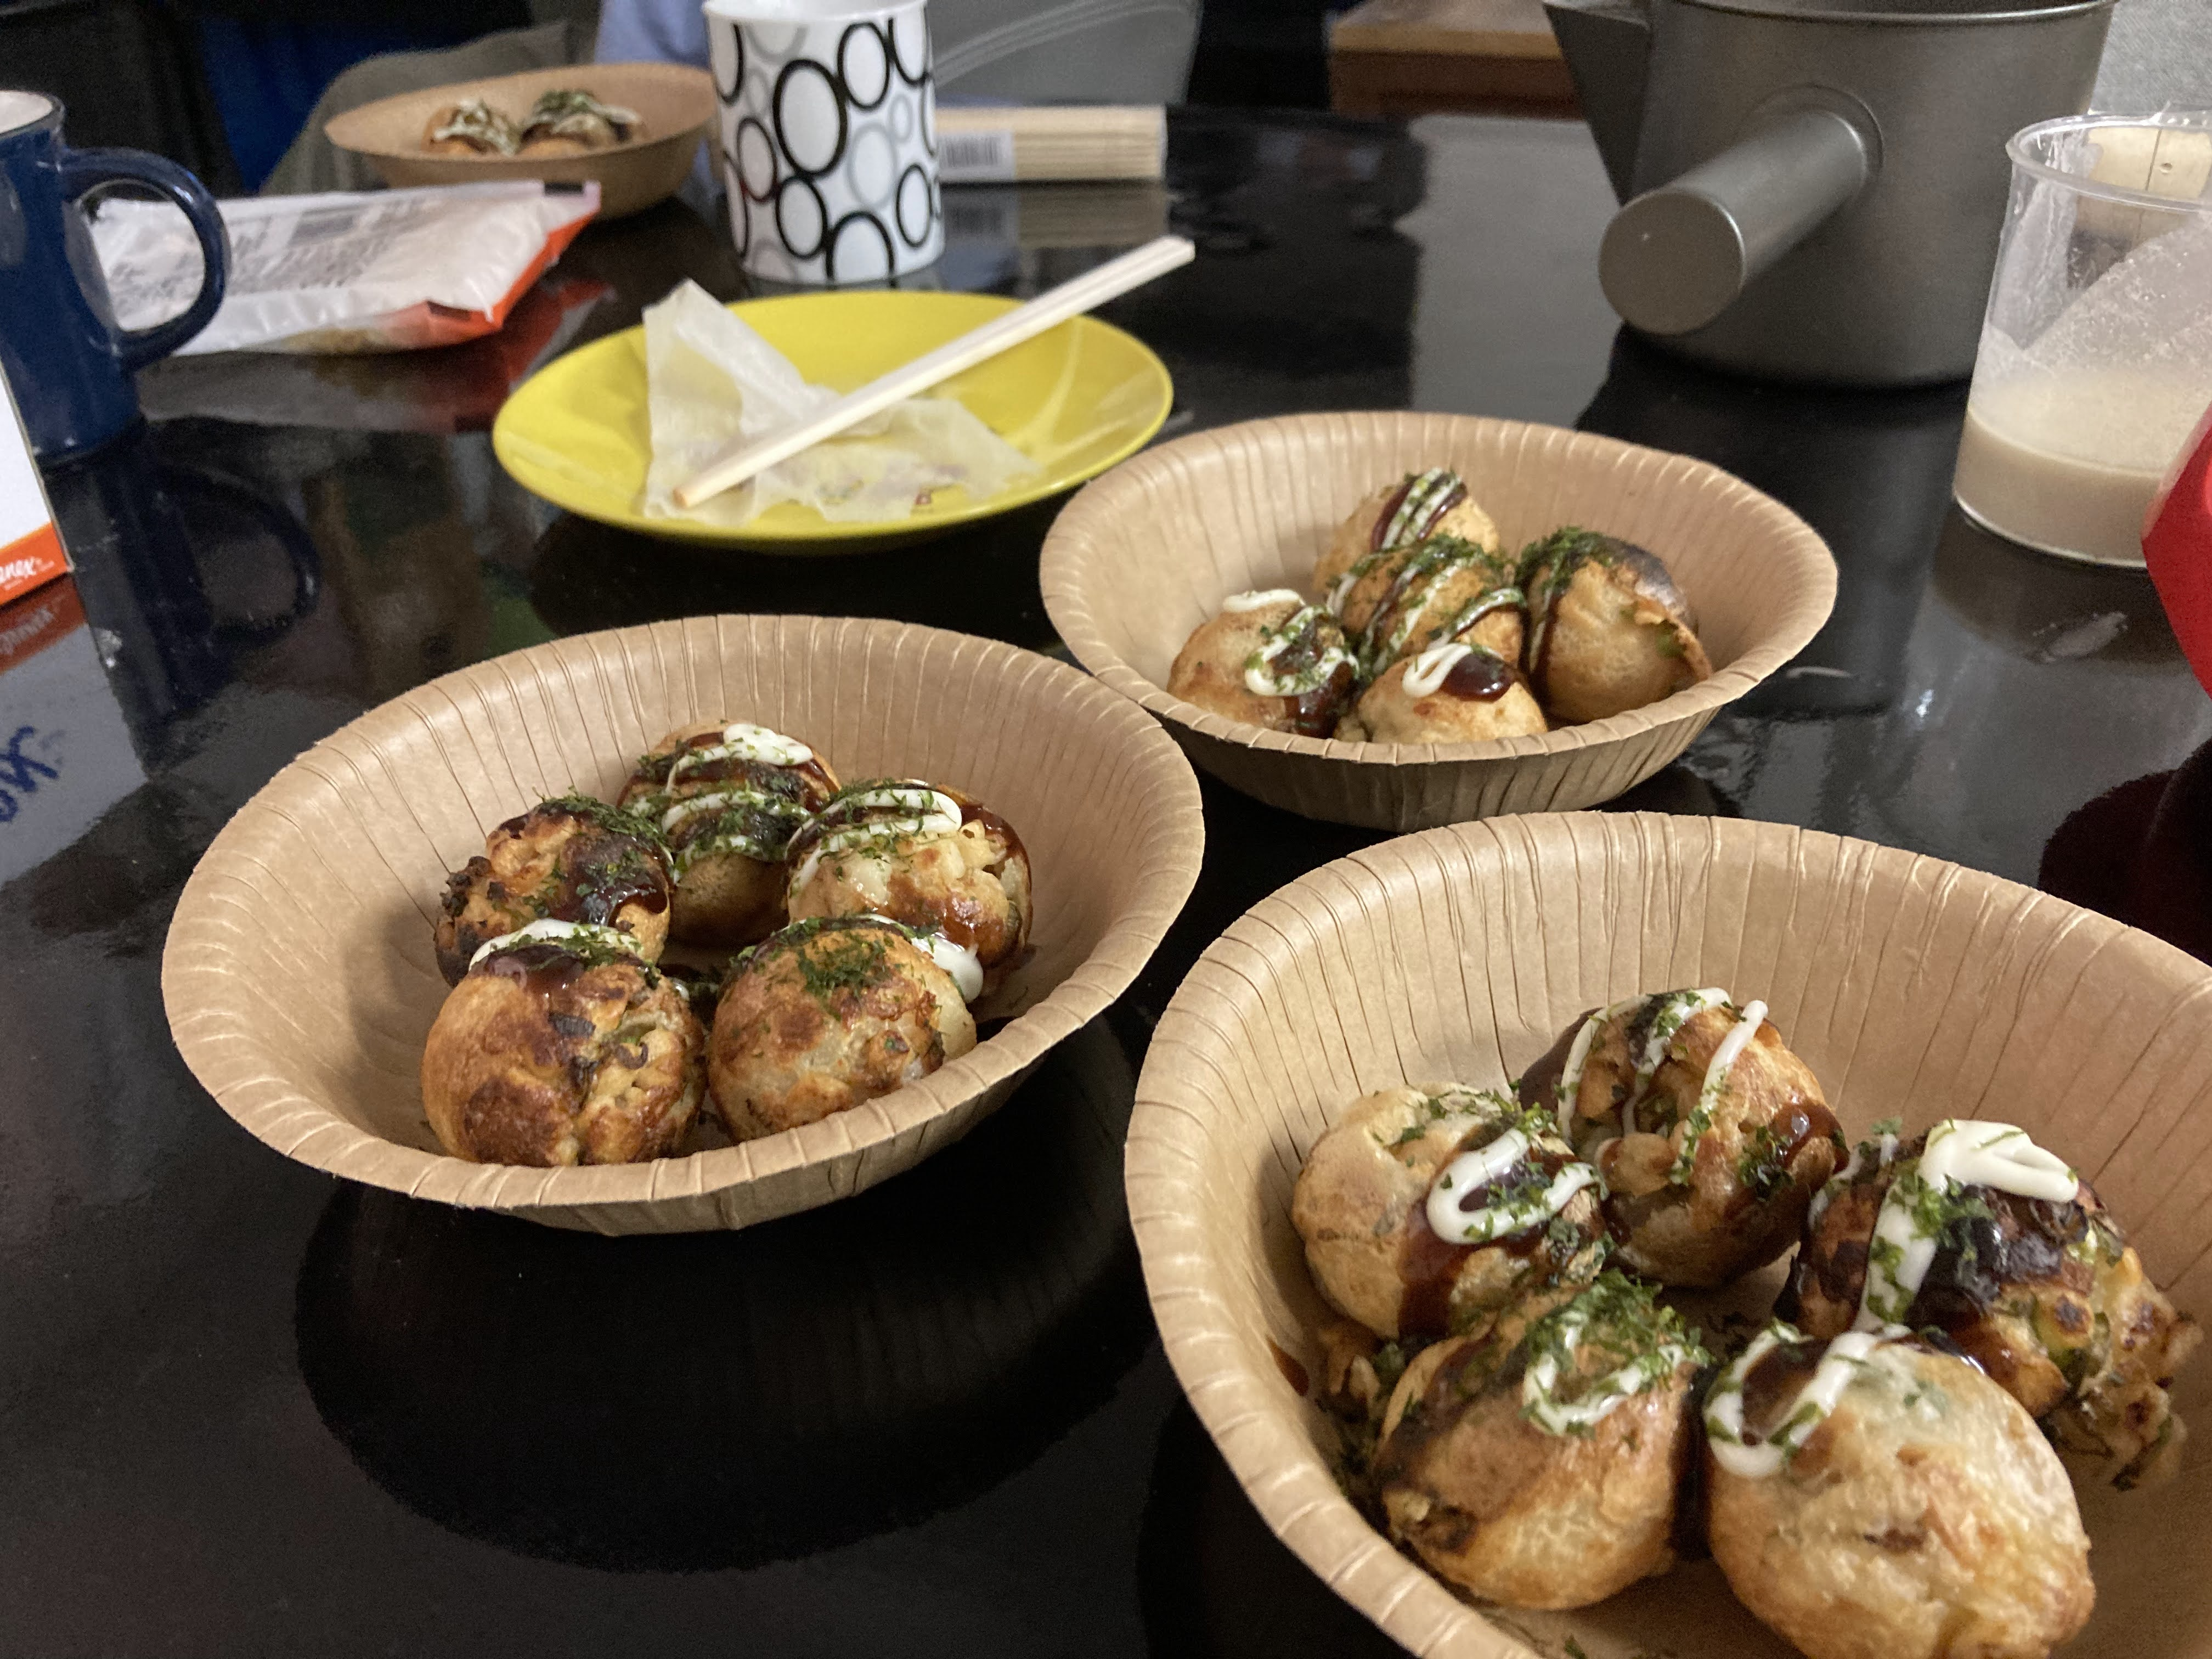
\includegraphics[width=6cm]{./image/04-Intarasting/takoyaki_soryusyon.jpg}
  \caption{たこ焼きでITをそりゅーしょんしている様子}
  \label{takoyaki_soryusyon}
\end{figure}
\chapter{これはchapter}
\section{これはsection}
我輩は猫である\footnote{こんな感じで脚注を書く}。

どこで生れたかとんと見当がつかぬ。何でも薄暗いじめじめした所でニャーニャー泣いていた事だけは記憶している。吾輩はここで始めて人間というものを見た。しかもあとで聞くとそれは書生という人間中で一番獰悪な種族であったそうだ。この書生というのは時々我々を捕えて煮て食うという話である。

\begin{tcolorbox}[breakable]
\begin{verbatim}
1  /* ここにはソースコードを書く */
2  #include<stdio.h>
3
4  int main(void)
5  {
6    printf("Hello, World!\n");
7    return 0;
8  }
9  /* breakableを付けるとこんな感じで改行にも対応できる */
\end{verbatim}
\end{tcolorbox}

\begin{shaded}
\begin{verbatim}
## ここにはコマンドを書く
$ echo "Hello, World!"
\end{verbatim}
\end{shaded}

図表はキャプションを付けたときに、先頭に「▲」や「▼」を付けるようにした。

\begin{table}[H]
  \centering
  \caption{表のサンプル}
  \begin{tabular}{|c|l|l|l|} \hline
    日本 & hoge & fuga & piyo \\ \hline
    アメリカ & foo & bar & baz \\ \hline
  \end{tabular}
  \label{table-sample0402}
\end{table}

\begin{figure}[H]
  \centering
  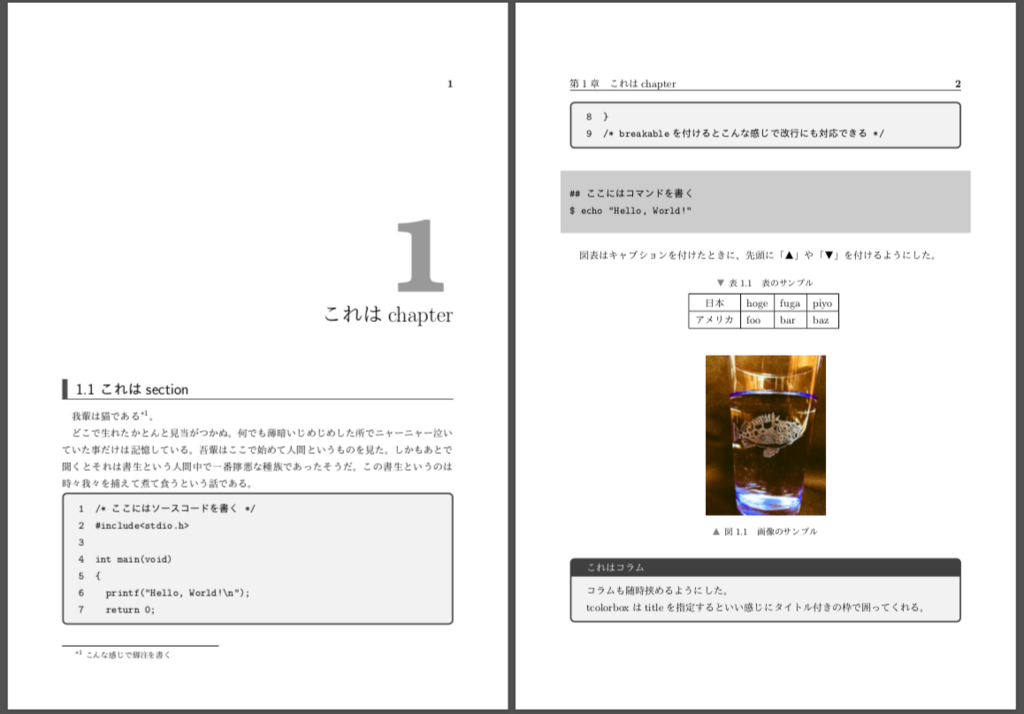
\includegraphics[width=4cm]{image/sample.png}
  \caption{画像のサンプル}
  \label{figure-sample0402}
\end{figure}

\begin{tcolorbox}[title=これはコラム]
  コラムも随時挟めるようにした。

  tcolorboxはtitleを指定するといい感じにタイトル付きの枠で囲ってくれる。
\end{tcolorbox}
\newpage
\thispagestyle{empty}
\section*{奥付け}

今回はこの本を手に取っていただきありがとうございました。
企画・編集を行いました、牧野です。
さて、六年ほど前のシス研では、本という形で技術をアウトプットするという文化があったと先輩から教えてもらいました。
今では、QiitaやZennのような技術ブログが発達して、物理的なもので残す文化がちょっとずつ廃れてしまったらしいです。
そんな中、私がC101の冬コミで技術本というものに出会いました、一つ一つ個人で調べたり研究した情報を、本という形で残すことにとてもいいと思い、今回このような本を執筆しました。
本というものは知識としてずっと蓄えられるものですので、私たちが書いた本が誰かの役にたてればと思い、締めさせてもらいます。
次回も余裕があれば出したいな。

企画・編集 牧野遥斗

\begin{table}[b]%
	\centering%
	\begin{tabular}{lcll}%
		\multicolumn{4}{c}{ {\LARGE Syskenの技術本 様々な技術を詰め合わせてみました。} }	\\
		\bhline{1pt}
		発行日 && 2023年 5月 28日 & (初版)	\\
%		 && 2019年 $\phantom{1}$2月 28日 &	(第二版)\\
		サークル && 愛知工業大学 システム工学研究会 &	\\
    Instagram ID && @ait.sysken& 	\\
		Twitter ID && @set$\_$official &	\\
		QiitaOrganizationURL && https://qiita.com/organizations/sysken &	\\
		代表 && 牧野遥斗 & \\
		代表者メールアドレス && harutiro2027@icloud.com & \\
		企画・編集 && 牧野遥斗 (Twitter: @minesu1224)  &	\\
		著者 && 林航平  &	\\
		   && すださんかり  &	\\
		   && hihumikan  &	\\
		   && Beyond Toyama  &	\\
		   && 水谷祐生 (Twitter @l8ZAFNZbON1eDbZ)  &	\\
		   && BlacKnight松土 (Twitter:@kk22blacknight)  &	\\
		   && shirataki1126  &	\\
		印刷所 && しまや出版 & \\
		\bhline{1pt}
		\multicolumn{4}{c}{ {※本書の無断複写、複製、データ配信はかたくお断りいたします。} }	
	\end{tabular}%
\end{table}%




\end{document}